\documentclass[10pt]{amsart}
\usepackage[a4paper,margin=23mm]{geometry}
\usepackage{amsmath,amssymb,amsthm,mathtools,hyperref,graphicx,xspace,letltxmacro,xpatch}
\usepackage[english]{babel}
\newtheorem{theo}{Theorem}[section]
\newtheorem{lemm}[theo]{Lemma}\newtheorem{prop}[theo]{Proposition}\newtheorem{coro}[theo]{Corollary}\newtheorem{conj}[theo]{Conjecture}
\theoremstyle{definition}\newtheorem{defi}[theo]{Definition}\newtheorem{rema}[theo]{Remark}\newtheorem{exam}[theo]{Example}\newtheorem{exem}[theo]{Example}\newtheorem{nota}[theo]{Notation}
\newcommand{\ie}{i.e.}\newcommand{\eg}{e.g.}\newcommand{\resp}{resp.}\newcommand{\skpt}{\par\smallskip\noindent}
\emergencystretch=3em\pagestyle{plain}

\usepackage{fancybox}
\usepackage{framed}
%\usepackage{enumerate}



 	


\newcommand{\RR}{\mathbb{R}}
\newcommand{\NN}{\mathbb{N}}
\newcommand{\CC}{\mathbb{C}}
\newcommand{\TT}{\mathbb{T}}
\renewcommand{\SS}{\mathbb{S}}

\newcommand{\Cc}{\mathcal{C}}
\newcommand{\Ac}{\mathcal{A}}
\newcommand{\Bc}{\mathcal{B}}
\newcommand{\Fc}{\mathcal{F}}
\newcommand{\Lc}{\mathcal{L}}
\newcommand{\Pc}{\mathcal{P}}
\newcommand{\Qc}{\mathcal{Q}}
\newcommand{\Oc}{\mathcal{O}}
\newcommand{\drm}{\mathrm{d}}

\DeclarePairedDelimiter{\VERT}{|\mkern -1.6mu|\mkern -1.6mu|}{|\mkern -1.6mu|\mkern -1.6mu|}

%\newcommand{\Kc}{\mathcal{K}}
%\newcommand{\Uc}{\mathcal{U}}
%\newcommand{\Vc}{\mathcal{V}}
%\newcommand{\Wc}{\mathcal{W}}
%\newcommand{\Nc}{\mathcal{N}}


\newcommand{\grad}{\nabla}
\renewcommand{\div}{\operatorname{div}}
\newcommand{\cnvh}{convhull}

%{c}
\newcommand{\vect}[2]{\left(
\begin{matrix} #1 \\ #2
\end{matrix}\right)}
\newcommand{\trans}{{^{\intercal}}}

\newcounter{stepcount}
%%\renewcommand{\thestepcount}{\alph{stepcount}}
\newenvironment{step}{\refstepcounter{stepcount}\begin{proof}[Step~\thestepcount]}{\let\qed\relax\end{proof}}



%\newdimen\texpscorrection
%\texpscorrection=0truecm
%\newdimen\figcenter
%\newcommand*\figurewithtex [1] #2 #3 #4 #5\\\null \goodbreak\figcenter=\hsize\relax
%\advance\figcenter by -#4truecm
%\divide\figcenter by 2
%
%\begin{figure}[hbt]
%\vskip #3truecm\noindent\hskip\figcenter
%\special{psfile=#1}{\hskip\texpscorrection\failedinput{\baselineskip=0.8\baselineskip
%\noindent \vbox{\noindent {\footnotesize #5}}\end{figure}}}
%\newcommand*\point[1] #2 #3 {\rlap{\kern #1 truecm\raise #2 truecm \hbox{#3}}}




%%%%%%%%%%%%%%%%%%%%%%%%%%%%%%%%%%%%%%%%%%%%%%%%%


\graphicspath{{./figures/}}

\newcommand*{\mk}{\mkern -1mu}
\newcommand*{\Mk}{\mkern -2mu}
\newcommand*{\mK}{\mkern 1mu}
\newcommand*{\MK}{\mkern 2mu}

\hypersetup{urlcolor=purple, linkcolor=blue, citecolor=red}

\newcommand*{\romanenumi}{\renewcommand*{\theenumi}{\roman{enumi}}}
\newcommand*{\Romanenumi}{\renewcommand*{\theenumi}{\Roman{enumi}}}
\newcommand*{\alphenumi}{\renewcommand*{\theenumi}{\alph{enumi}}}
\newcommand*{\Alphenumi}{\renewcommand*{\theenumi}{\Alph{enumi}}}
\let\oldtilde\tilde
\renewcommand*{\tilde}[1]{\mathchoice{\widetilde{#1}}{\widetilde{#1}}{\oldtilde{#1}}{\oldtilde{#1}}}\let\oldexists\exists
\renewcommand*{\exists}{\mathrel{\oldexists}}
\let\oldforall\forall
\renewcommand*{\forall}{\mathrel{\oldforall}}

%%%%%%%%%%%%%%%%%%%%%%%%%%%%%%%%%%%%%%%%%%%%%%%%
\newtheorem{lemma}[theo]{Lemma}
\newenvironment{remas}[1][]{\begin{rema}[#1]}{\end{rema}}
\title{Polynomial and stretched-exponential decay-rate transfer for stabilized semilinear damped waves}
\author{Joly, Romain, Laurent, Camille}
\date{doi:10.5802/ahl.60; CC BY 4.0}
\begin{document}
\maketitle
\noindent\textit{Editorial note.} Only selected author result counted; complete original mathematical body and bibliography preserved. Complete native vector PDF Forms with nested graphics resources retained; original proof-step macros preserved.\par\medskip
\noindent\textit{Allowed standard prerequisites (editorial).}\begin{itemize}
\item Standard functional analysis, measure theory and the author-cited classical theorems. Standard prior results stay cited; complete source-local proofs and definitions retained.
\end{itemize}\medskip


\section{Introduction}

We consider the semilinear damped wave equation
\begin{equation}\label{eq}
\begin{cases}
\partial_{tt}^2 u + \gamma(x)\partial_t u = \Delta u - \alpha u - f(x,u)\:&(x,t)\in\Omega\times (0,+\infty)\\
u_{|\partial\Omega}(x,t)=0&(x,t)\in\partial\Omega\times (0,+\infty)\\
\left(u(\cdot,t=0),\partial_t u(\cdot,t=0)\right)=U_0=(u_0,u_1)& \mkern43mu\in H^1_0(\Omega)\times L^2(\Omega)
\end{cases}
\end{equation}
in the following general framework:
\begin{enumerate}\romanenumi
\item \label{listintro1.1}the domain $\Omega$ is a two-dimensional smooth compact and connected manifold with or without smooth boundary. If $\Omega$ is not flat, $\Delta$ has to be taken as Beltrami Laplacian operator.
\item \label{listintro1.2}the constant $\alpha\geq 0$ is a non-negative constant. We require that $\alpha>0$ in the case without boundary to ensure that $\Delta-\alpha Id$ is a negative definite self-adjoint operator.
\item \label{listintro1.3}the damping $\gamma\in L^\infty(\Omega,\RR_+)$ is a bounded function with non-negative values. Since we want to consider a damped equation, we will assume that $\gamma$ does not vanish everywhere.
\item \label{listintro1.4}the non-linearity $f\in\Cc^1(\overline\Omega\times\RR,\RR)$ is of polynomial type in the sense that there exists a constant $C$ and a power $p\geq 1$ such that for all $(x,u)\in \overline\Omega\times\RR$,
\begin{equation}\label{hyp-f-estim}
|f(x,u)|+|\grad_xf(x,u)|\leq C(1+|u|)^p\:\text{ and }\:|f'_u(x,u)|\leq C(1+|u|)^{p-1}\,.
\end{equation}
Moreover, in most of this paper, we will be interested in the stabilization problem and we will also assume that
\begin{equation}\label{hyp-f-sign}
\forall (x,u)\in \overline\Omega\times\RR\,,\:f(x,u)u\geq 0\,.
\end{equation}
\end{enumerate}


We introduce the space $X=H^1_0(\Omega)\times L^2(\Omega)$ and the operator $A$ defined by
\[
D(A)=\left(H^2(\Omega)\cap H^1_0(\Omega)\right)\times H^1_0(\Omega)\quad
A =
\begin{pmatrix}
0 & Id \\
\Delta-\alpha Id & -\gamma(x)
\end{pmatrix}\,.
\]
In this paper, we are interested in the cases where the linear semigroup $e^{At}$ has no uniform decay, that is that $\|e^{At}\|_{\Lc(X)}$ does no converge to zero. We only assume a semi-uniform decay, but sufficiently fast in the following sense.

\begingroup
\begin{enumerate}\romanenumi
\setcounter{enumi}{4}
\item \label{listintro1.5}There exists a function $h(t)$ such that
\begin{equation}\label{hyp-decay-1}
\forall U_0\in D(A)\,,\,\left\|e^{At}U_0\right\|_X \, \leq \, h(t)\,\|U_0\|_{D(A)}
\end{equation}
and there is $\sigma_h\in(0,1]$ such that
\begin{equation}\label{hyp-decay-2}
\lim_{t\rightarrow \infty}h(t)=0\;\text{ and }\,
\forall \sigma\in[0,\sigma_h]\,,\:\int_0^\infty h(t)^{1-\sigma}\,\drm t\,<\,\infty\,.
\end{equation}
\end{enumerate}
\endgroup
Condition~\eqref{hyp-decay-2} requires a decay rate fast enough to be integrable. Roughly speaking, this article shows that this condition, together with a suitable unique continuation property, are sufficient to obtain a stabilization of the semilinear equation. The relevant unique continuation property is explained in Proposition~\ref{prop-UCP-implique-th} below. We present two general results where it can be obtained.

Our first result concerns analytic nonlinearities and smooth dampings.

\begin{theo}\label{th1}
Consider the damped wave equation~\eqref{eq} in the framework of Assumptions~\eqref{listintro1.1}-\eqref{listintro1.5}. Assume in addition that:
\begin{enumerate}\alphenumi
\item \label{listtheo1.1.1}the function $(x,u)\mapsto f(x,u)$ is smooth and analytic with respect to $u$.
\item \label{listtheo1.1.2}the damping $\gamma$ is of class $\Cc^1$ or at least that there exists $\tilde\gamma\in\Cc^1(\overline\Omega,\RR_+)$ such that~\eqref{listintro1.5} holds with $\gamma$ replaced by $\tilde\gamma$ and such that the support of $\tilde\gamma$ is contained in the support of $\gamma$.
\item \label{listtheo1.1.3}the power $p$ of $f$ in~\eqref{hyp-f-estim} and the decay rate $h(t)$ of the semigroup in~\eqref{hyp-decay-1} satisfy $h(t)=\Oc(t^{-\beta})$ with $\beta>2p$.
\end{enumerate}
Then, any solution $u$ of~\eqref{eq} satisfies
\[
\|(u,\partial_t u)(t)\|_{H^1_0\times L^2}\,\xrightarrow[\:t\longrightarrow
+\infty\:]{}\,0\,.
\]
Moreover, for any $R$ and $\sigma>0$, there exists $h_{R,\sigma}(t)$ which goes to zero when $t$ goes to $+\infty$ such that the following stabilization hold. For any $U_0\in H^{1+\sigma}_0(\Omega)\times H^\sigma(\Omega)$, if $u$ is the solution of~\eqref{eq}, then
\[
\|(u_0,u_1)\|_{H^{1+\sigma}\times H^\sigma}\leq
R\:\Longrightarrow\:\|(u,\partial_t u)(t)\|_{H^1_0\times L^2} \leq
h_{R,\sigma}(t)\,\xrightarrow[\:t\longrightarrow +\infty\:]{}\,0\,.
\]
\end{theo}

Our assumptions~\eqref{listintro1.5} and~\eqref{listtheo1.1.3} on the decay of the linear semigroup may seem strong. They are satisfied in the cases where the set of trapped geodesics, the ones which do not meet the support of the damping, is small and hyperbolic in some sense. Several geometries satisfying~\eqref{listintro1.5} and~\eqref{listtheo1.1.3} have been studied in the literature, see the concrete examples of Figure~\ref{fig-1} and the references therein. Notice in particular that the example of domain with holes is particularly relevant for applications where we want to stabilize a nonlinear material with holes by adding a damping or a control in the external part. There is a huge literature about the damped wave equation and the purpose of the examples presented here is mainly to illustrate our theorem to non specialists. Moreover, the subject is growing quickly, giving more and more examples of geometries where we understand the effect of the damping and where we may be able to apply our results. We do not pretend to exhaustivity and refer to the bibliography of the more recent~\cite{Lin} for instance.

In some cases, the unique continuation property required in Proposition~\ref{prop-UCP-implique-th} can be obtained without considering analytic nonlinearities or conditions on the growth of $f$ as Hypothesis c) of Theorem~\ref{th1}. Instead, we require a particular geometry, which will be introduced more precisely in Section~\ref{section-UCP}.
\goodbreak

\begin{theo}\label{th2}
Consider the damped wave equation~\eqref{eq} in the framework of Assumptions~\eqref{listintro1.1}-\eqref{listintro1.5}. Assume in addition that:
\begin{enumerate}\alphenumi
\item \label{listtheo1.2.1}the function $(x,u)\mapsto f(x,u)$ is of class $\Cc^1\left(\overline{\Omega}\times \RR,\RR\right)$.
\item \label{listtheo1.2.2}there exists a pseudo-convex foliation of $\Omega$ in the sense of Definitions~\ref{defi-foliation1} or~\ref{defi-foliation2}.
\end{enumerate}
Then, the conclusions of Theorem~\ref{th1} hold.
\end{theo}

This result can be applied in several situations of Figure~\ref{fig-1}: the ``disk with two holes'', the ``peanut of rotation'' and the ``open book''. In these cases, the stabilization holds for any natural nonlinearity.

We expect that the decay rate $h_{R,\sigma}(t)$ is related to the linear decay rate $h(t)$ of Assumption~\eqref{listintro1.5}. We are able to obtain this link for the typical decays of the examples of Figure~\ref{fig-1}.


\begin{prop}\label{prop1}
Consider a situation where the stabilization stated in Theorems~\ref{th1} or~\ref{th2} holds. Then,
\begin{itemize}
\item if the decay rate of Assumption~\eqref{listintro1.5} satisfies $h(t)=\Oc({t^{-\alpha}})$ with $\alpha>1$, then the nonlinear equation admits a decay of the type $h_{R,\sigma}(t)= \Oc (t^{-\sigma\alpha})$.
\item if the decay rate of Assumption~\eqref{listintro1.5} satisfies $h(t)=\Oc \left(e^{-a {t^{1/\beta}}}\right)$ with $a>0$ and $\beta>0$, then the nonlinear equation admits a decay of the type $h_{R,\sigma}(t)\linebreak= \Oc \left(e^{-b\sigma t^{1/(\beta+1)}}\right)$ for some $b>0$.
\end{itemize}
\end{prop}


Notice that this result is purely local in the sense that the decay rate is obtained when the solution is close enough to $0$. Our proofs do not provide an explicit estimate of the time needed to enter this small neighborhood of $0$. Also notice that the loss in the power of the second case of Proposition~\ref{prop1} is due to an abstract setting: in the concrete examples, we may avoid this loss, see the remark below Lemma~\ref{lemma-appli2} and the concrete applications to the examples of Figure~\ref{fig-1}.

{\small
\begin{figure}[tp]
%\ovalbox{
\begin{minipage}{14cm}
\begin{minipage}{4.3cm}
%remplacer les box par env approprié !
{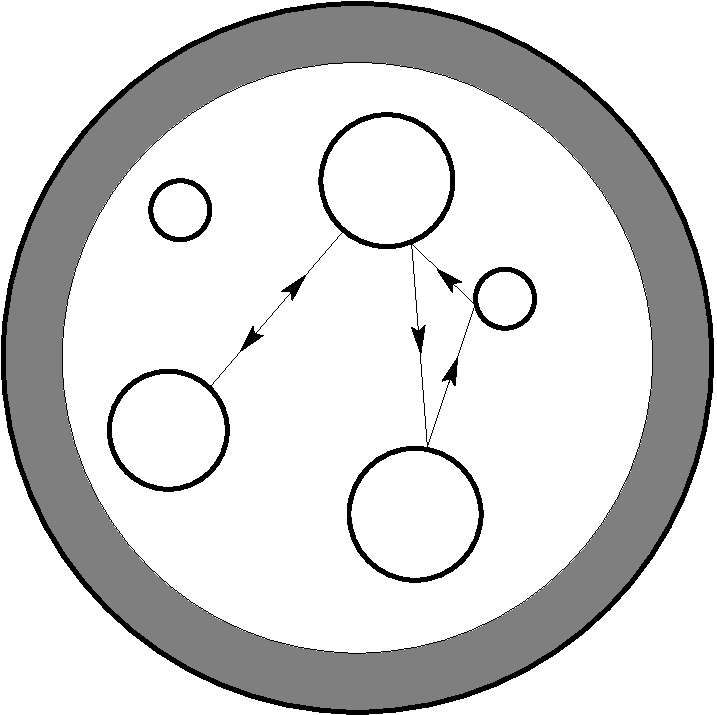
\includegraphics[scale=0.35]{Figures/disque-trous.pdf} }
\end{minipage}
\begin{minipage}{9cm}
{\bf Disk with holes}\\
We set $\Omega$ to be a convex flat surface with a damping $\gamma$ efficient near the boundary. Typically, we may take the flat disk $B(0,1)$ of $\RR^2$ and assume that there exist $r\in(0,1)$ and $\underline\gamma>0$ such that $\gamma(x)\geq \underline\gamma>0$ for $|x|>r$. Inside the interior zone without damping, assume that at least two holes exist; to simplify, we also assume that these holes are disks and are small in a sense specified later. Notice that there exist some periodic geodesics which do not meet the support of the damping. This example has been studied in~\cite{Burq-memoire, Burq-Zworski}.
\end{minipage}
\end{minipage}
%}

\vspace{1mm}

%\ovalbox{
\begin{minipage}{14cm}
\vspace{1mm}
\begin{minipage}{7cm}
{\bf The peanut of rotation}\\
We consider a compact two-dimensional manifold without boundary. We assume that the damping $\gamma$ is effective, that is uniformly positive, everywhere except in the central part of the manifold. This part is a manifold of negative curvature and
\end{minipage}
\begin{minipage}{6.8cm}
\begin{center}
{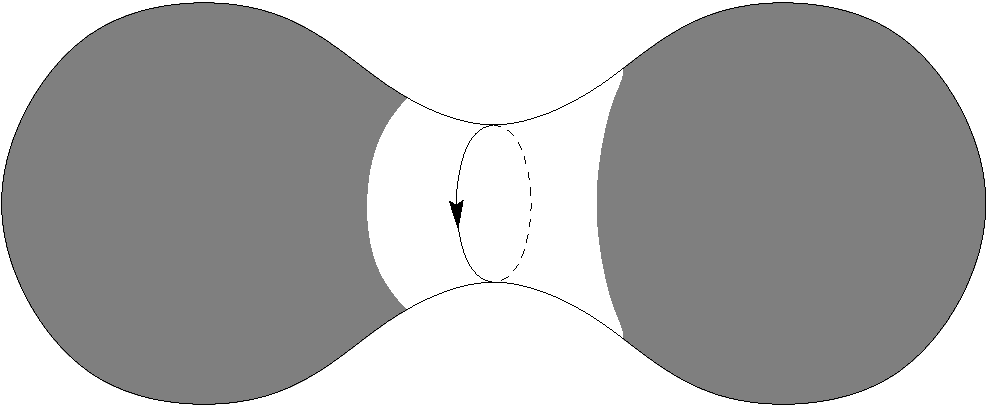
\includegraphics[scale=0.25]{Figures/revolution-peanut.pdf} }
\end{center}
\end{minipage}\\[1mm]
invariant by rotation along the $y-$axis. More precisely, let us set this part to be equivalent to the cylinder endowed with the metric $g(y,\theta)=\drm y^2+\cosh^2(y)\drm\theta^2$. This central part admits a unique (up to change of orientation) periodic geodesic which is unstable; any other geodesic meets the support of the damping. This example has been studied for example in~\cite{CSVW,Schenck} and the references therein.\\[-4mm]
\end{minipage}
%}

\vspace{1mm}

%\ovalbox{~
\begin{minipage}{14cm}
\begin{minipage}{4.1cm}
{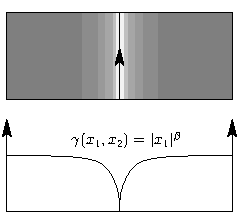
\includegraphics{Figures/open-book-legende.pdf}}
\end{minipage}
\begin{minipage}{9.5cm}
$~$\\
{\bf The open book}\\
We consider the torus $\TT^2$ with flat geometry. The damping $\gamma$ is assumed to depend only on the first coordinate and to be of the type $\gamma(x)=|x_1|^\beta$ with $\beta>0$ to be chosen small enough. In this case, there is a unique (up to change of orientation) geodesic which does not meet the support of the damping. This example has been studied in~\cite{Leautaud-Lerner}.\\
\end{minipage}
\end{minipage}
%$~~$}


\vspace{1mm}

%\ovalbox{~
\begin{minipage}{14cm}
\begin{minipage}{7cm}
\vspace{1.5mm}
{\bf Hyperbolic surfaces}\\
We consider a compact connected hyperbolic surface with constant negative curvature -1 (for example a surface of genus 2 cut out from Poincaré disk). The damping is any non zero function $\gamma(x)\geq 0$. This example has been studied in~\cite{Lin} following the fractal uncertainty principle of~\cite{BourgainDyatlov}. We also refer to other results in any dimension with pressure conditions~\cite{Riv,Schenckpressure} following ideas of~\cite{Anant}.\\
$~$
\end{minipage}
\begin{minipage}{6.2cm}
{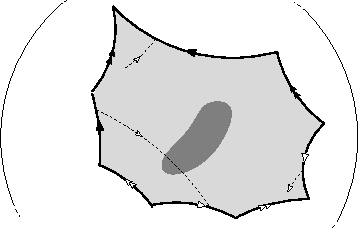
\includegraphics[scale=1.05]{Figures/hyperbo2.pdf} }
\end{minipage}
\end{minipage}
%$\MK$}
\caption{The main applications of Theorems~\ref{th1} and~\ref{th2} presented in this paper. The gray parts show the localization of the damping (white = no damping). The more geometrically constrained Theorem~\ref{th2} apply to the ``disk with two holes'', the ``peanut of rotation'' and the ``open book''. \label{fig-1}}
\end{figure}}

%\vspace{3mm}


To our knowledge, Theorems~\ref{th1} and~\ref{th2} are the first stabilization results for the semilinear damped wave equation when the geometric control condition fails. This famous geometric control condition has been introduced in the works of Bardos, Lebeau, Rauch and Taylor (see~\cite{BLR}) and roughly requires that any geodesic of the manifold $\Omega$ meets the support of the damping $\gamma$. This condition implies that the linear semigroup of the damped wave equation satisfies a uniform decay $\|e^{At}\|_{\Lc(H^1_0\times L^2)}\leq Me^{-\lambda t}$. In this context, the stabilization of the semilinear damped wave equation has been studied since a long time, see for example~\cite{Dehman,DLZ,Haraux,RC, Zuazua}. Under this condition and for large data, the proof often divides into a part dealing with high frequencies with linear arguments and another one dealing with low frequencies that often requires a unique continuation argument. The high frequency problem was solved by Dehman~\cite{Dehman} with important extension by Dehman--Lebeau--Zuazua~\cite{DLZ} using microlocal defect measure. Yet, the unique continuation was proved by classical Carleman estimates (see Section~\ref{subsectUCPwithout} below) which restricted the generality of the geometry. Using techniques from dynamical systems applied to PDEs, the authors of the present article proved in~\cite{RC} a general stabilization result under Geometric Control Condition, at the cost of an assumptions of analyticity of the nonlinearity. Theorem~\ref{th1} is in the same spirit as~\cite{RC} and intends to prove that related techniques can be extended to a weaker damping. Theorem~\ref{th2} is more in the spirit of the other references, taking advantage of particular geometries, but avoiding analyticity.


Notice that the ``disk with one hole'' satisfies this geometric control condition and thus it is not considered in this paper.

In the cases where the geometric control condition fails, the decay of the linear semigroup is not uniform. At least, if $\gamma$ does not vanish everywhere, it is proved in~\cite{Dafermos} (see also~\cite{Haraux}) that the trajectories of the linear semigroup go to zero (see Theorem~\ref{th-stab-linear} below). In fact, the decay can be estimated with a loss of derivative as
\begin{equation}\label{eq-weak-decay}
\left\|e^{At}U\right\|_{H^1\times L^2}\,\leq\, h(t)
\|U\|_{H^2\times H^1}\quad\text{with}\quad h(t)\xrightarrow[\,t\rightarrow +\infty\,]{} 0\,.
\end{equation}
In the general case, as soon as $\gamma\not\equiv 0$, the decay rate can be taken as\linebreak$h(t)=\Oc(\ln(\ln(t))/\ln t)$ as shown in~\cite{Lebeau,Lebeau-Robbiano}. In some particular situations, $\gamma$ misses the geometric control condition but very closely: typically there is only one (up to symmetries) geodesic which does not meet the support of the damping and this geodesic is unstable. In this case, we may hope a better decay than the $\Oc(\ln(\ln(t))/\ln t)$ one, see for example~\cite{CSVW,Leautaud-Lerner} and the other references of Figure~\ref{fig-1}.

To our knowledge, until now, there was no result concerning the semilinear damped wave equation~\eqref{eq} when the geometric control condition fails. Thus Theorems~\ref{th1} and~\ref{th2} provides the first examples of semi-uniform stabilization for the semilinear damped wave equation. Notice that our results deeply rely on the fact that the decay rate of~\eqref{eq-weak-decay} is integrable. Typically, for the situations of Figure~\ref{fig-1}, it is of the type $h(t)=\Oc(e^{-\lambda t^\alpha})$ or $h(t)=\Oc(1/t^\beta)$ with sufficiently large $\beta>0$.

%\vspace{3mm}

Theorems~\ref{th1} and~\ref{th2} concern the stabilization of the solutions of~\eqref{eq} in the sense that their $H^1\times L^2$-norm goes to zero. Notice that, since the energy of the damped wave equation is non-increasing (see Section~\ref{section-basic}), we knew that this $H^1\times L^2$-norm is at least bounded. Such a uniform bound is not clear a priori for the $H^2\times H^1$-norm. However, basic arguments provide this bound as a corollary of Theorems~\ref{th1} and~\ref{th2} if the decay is fast enough, which is the case of the ``disk with holes'', the ``peanut of rotation'' and the ``hyperbolic surfaces'' of Figure~\ref{fig-1}.

\begin{theo}\label{th-norm-H2}
Consider the damped wave equation~\eqref{eq} in the framework of Theorems~\ref{th1} or~\ref{th2}. Assume that for all $R>0$, the decay rate $h_{R,1}(t)$ is faster than polynomial, i.e. $h_{R,1}(t)=o(t^{-k})$ for any $k\in\NN$. Also assume that $\gamma$ is of class $\Cc^1$ and $f$ is of class $\Cc^2(\overline\Omega\times \RR,\RR)$. Then the $H^2(\Omega)\times H^1(\Omega)$-norm of the solutions are bounded in the following sense. For any $R>0$, there exists $C(R)>0$ such that, for any $U_0\in (H^{2}(\Omega)\cap H^1_0(\Omega))\times H^1_0(\Omega)$ such that $\|U_0\|_{H^2\times H^1} \leq R$, the solution $u$ of~\eqref{eq} satisfies
\[
\sup_{t\geq 0} \|(u,\partial_t u)(t)\|_{H^2\times H^1} \leq C(R)\,.
\]
\end{theo}

Note that, in the case without damping, this result is sometimes expected to be false. It is related to the weak turbulence, described as a transport from low frequencies to high frequencies, see~\cite{Colliander,Gerard-Grellier,Hani}.


%\vspace{3mm}

The main purpose of this paper is to obtain new examples of stabilization for the semilinear damped wave equation and to introduce the corresponding methods and tools. We do not pretend to be exhaustive and the method may be easily used to obtain further or more precise results. For example:
\begin{itemize}
\item the boundary condition may be modified, typically in the case of the disk with holes, Neumann boundary condition may be chosen at the exterior boundary.
\item for simplicity, the examples of Figure~\ref{fig-1} and the main results of this article concern two-dimensional manifolds. However, the arguments of this paper can be used to deal with higher-dimensional manifolds. There are some technical complications, mainly due to the Sobolev embeddings. For example, in dimension $d=3$, the degree of $f$ in~\eqref{hyp-f-estim} should satisfy $p<3$ ($p<5$ if we use Strichartz estimates as done in~\cite{RC} using~\cite{DLZ}) and the order $\beta$ of the vanishing of $\gamma$ in the example of the open book should not be too large. To simplify, we choose to state our results in dimension $d=2$. However, several intermediate results in this article are stated for dimensions $d=2$ or $d=3$.
\item It is also possible to combine the strategy of this paper with other tricks and technical arguments. For example, we may consider unbounded manifolds or manifolds of dimension $d=3$ with nonlinearity of degree $p\in [3,5)$, which are supercritical in the Sobolev sense. This would requires to use Strichartz estimates in addition to Sobolev embeddings as done in~\cite{Dehman}, \cite{DLZ} or~\cite{RC}.
\item assume that we replace the sign condition~\eqref{hyp-f-sign} by an asymptotic sign condition
\[
\exists R>0\,,\:\forall (x,u)\in
\overline\Omega\times\RR\,,\:|u|\geq R\,\Rightarrow\,f(x,u)u\geq 0\,.
\]
Then they may exist several equilibrium points and the stabilization to zero cannot be expected. However, the arguments of this paper show that the energy $E$ introduced in Section~\ref{section-basic} is a strict Lyapounov functional and that any solution converges to the set of equilibrium points. We can also show the existence of a \emph{weak compact attractor} in the sense that there is an invariant compact set $\Ac\subset H^1_0(\Omega)\times L^2(\Omega)$, which consists of all the bounded trajectories and such that any regular set $\Bc$ bounded in $(H^2(\Omega)\cap H^1_0(\Omega))\times H^1_0(\Omega)$ is attracted by $\Ac$ in the topology of $H^1_0(\Omega)\times L^2(\Omega)$. Notice that this concept of weak attractor is the one of Babin and Vishik in~\cite{Babin-Vishik}. At this time, the asymptotic compactness property of the semilinear damped wave equation was not discovered and people thought that a strong attractor (attracting bounded sets of $H^1_0(\Omega)\times L^2(\Omega)$) was impossible due to the lack of regularization property for the damped wave equation. Few years later, Hale~\cite{Hale-book} and Haraux~\cite{Haraux} obtained this asymptotic compactness property and the existence of a strong attractor. Thus this notion of weak attractor has been forgotten. It is noteworthy that it appears again here. Notice that we cannot hope a better attraction property since even in the linear case, $\{0\}$ is not an attractor in the strong sense.
\end{itemize}

%\vspace{3mm}

The organization of this paper follows the proof of stabilization of the examples of Figure~\ref{fig-1}. We add step by step the techniques required to deal with our guiding examples, from the simplest to the most complicated one.

Sections~\ref{section-basic} and~\ref{section-asymp-compact} contain the basic notations and properties. The asymptotic compactness of the semilinear dynamics is proved and the problem is reduced to a unique continuation property. In Section~\ref{section-decay}, we show the estimations of Proposition~\ref{prop1}. Section~\ref{section-appli1} then proves the nonlinear stabilization in the ``open book'' case, where the unique continuation property is trivial. Section~\ref{section-UCP} stated several unique continuation results, enabling to prove Theorem~\ref{th2}. We obtain as a consequence the stabilization in the case of the ``peanut of rotation'' in Section~\ref{section-appli2}. Section~\ref{section-decay-disk} studies the linear semigroup for the case of the ``disk with holes'' before we apply Theorem~\ref{th2} in the case of the ``disk with two holes'' in Section~\ref{section-appli3}. Theorem~\ref{th1} is proved in Section~\ref{section-reg-analytic} by showing an asymptotic analytic regularization. It is applied to the ``disk with three or more holes'' and hyperbolic surfaces, assuming $f$ analytic in $u$, in Sections~\ref{section-appli4} and~\ref{section-hyperbo}. In Section~\ref{section-th-norm-H2}, we show how to obtain Theorem~\ref{th-norm-H2} as a corollary of Theorems~\ref{th1} or~\ref{th2}. This article finishes with three appendices on the links between the decay of the semigroup $e^{At}$ and the resolvent $(A-i\mu Id)^{-1}$.

\subsection*{Acknowledgements}
The authors deeply thank Matthieu Léautaud for his contributions to the appendices. They are also grateful to Nicolas Burq for several discussions and the suggestion of Theorem~\ref{th-norm-H2}.



\section{Notations and basic facts}\label{section-basic}
We use the notations of Equation~\eqref{eq}, of Assumptions~\eqref{listintro1.1}-\eqref{listintro1.5} and of the introduction. In particular, we recall that $X=H^1_0(\Omega)\times L^2(\Omega)$ and
\[
D(A)=\left(H^2(\Omega)\cap H^1_0(\Omega)\right)\times H^1_0(\Omega)\,
A =
\begin{pmatrix}
0 & Id \\ \Delta-\alpha Id & -\gamma(x)
\end{pmatrix}\,.
\]
The operator $A$ is the classical linear damped wave operator corresponding to the linear part of~\eqref{eq}. Due to Lumer--Phillips theorem, we know that this operator generates a linear semigroup of contractions $e^{At}$ on $X$ and on $D(A)$ and that
\[
\forall t\geq 0\,,\,\left\|e^{At}\right\|_{\Lc(X)}\leq 1\quad\text{and}\quad\left\|e^{At}\right\|_{\Lc(D(A))}\leq 1\,.
\]
Notice that the second estimate is a direct consequence of the commutation of $A$ and $e^{At}$ and does not require any regularity on $\gamma$.

For any $\sigma\in [0,1]$, we set
\[
X^\sigma=\left(H^{1+\sigma}(\Omega)\cap H^1_0(\Omega)\right)\times
H^\sigma_0(\Omega)\,.
\]
Thus $X^0=X$ and $X^1=D(A)$ and $X^\sigma$ is an interpolation space between $X^0$ and $X^1$. In particular, by interpolation, $e^{At}$ is defined in $X^\sigma$ and we have
\begin{equation}\label{eq-bound-semigroup}
\forall \sigma\in [0,1]\,,\:\forall t\geq 0\,,\:
\left\|e^{At}\right\|_{\Lc(X^\sigma)}\leq 1\,.
\end{equation}

We set $F\in\Cc^0(X)$ to be the function
\begin{equation}\label{def-F}
F:U=\vect uv \in X\,\longmapsto\,\vect 0 {-f(\cdot,u)} \in X\,.
\end{equation}
Notice that, if $\Omega$ is two-dimensional, $H^1_0(\Omega) \hookrightarrow L^{p}(\Omega)$ for any $p\in[1,+\infty)$ and if $\Omega$ is three-dimensional $H^1_0(\Omega) \hookrightarrow L^6(\Omega)$. Thus, $f(u)$ is well defined in $L^2(\Omega)$ due to Assumption~\eqref{hyp-f-estim} if dim$(\Omega)=2$ or if dim$(\Omega)=3$ and $p\leq 3$. Moreover, for any $R$, $u$ and $v$ with $\|u\|_{H^1}\leq R$ and $\|v\|_{H^1}\leq R$, we have
\[
\|f(\cdot,u)-f(\cdot,v)\|_{L^2}=\left\|(u-v)\int_0^1
f'_u(\cdot,u+s(u-v))ds\right\|_{L^2}
\leq C(R)\|u-v\|_{H^1}
\]
and so $F$ is lipschitzian on the bounded sets of $X$. As a consequence, the damped wave equation~\eqref{eq} is well posed in $X$ and admits local solutions if dim$(\Omega)=2$ or if dim$(\Omega)=3$ and $p\leq 3$.

With the above notation, our main equation writes
\begin{equation}\label{eq2}
\partial_t U=AU + F(U)\quad U(t=0)=U_0\in X\,.
\end{equation}
In particular, Duhamel's formula yields
\[
U(t)=e^{At}U_0 + \int_0^t e^{A(t-s)}F(U(s))\,\drm s\,.
\]

We introduce the potential
\[
V(x,u)=\int_0^u f(x,s)ds\,.
\]
Due to~\eqref{hyp-f-estim} and the above arguments, $V(\cdot,u)$ defines a Lipschitz function from the bounded sets of $H^1_0(\Omega)$ into $L^1(\Omega)$. The classical energy associated to~\eqref{eq} is defined along a trajectory $U=(u,\partial_t u)$ as
\[
E(U)= \int_\Omega \frac12\left(|\grad u|^2+\alpha |u|^2+|\partial_t u|^2\right) +
V(x,u)\,.
\]
The damping effect appears by the computation
\begin{equation}\label{eq-deriv-E}
\partial_t E(U(t))= - \int_\Omega \gamma(x)|\partial_t u |^2\,.
\end{equation}
In particular, the energy $E$ is non-increasing along the trajectories. Moreover, the sign assumption~\eqref{hyp-f-sign} yields that $V(x,u)\geq 0$. Thus, we have that $E(U)\geq C \|U\|_X^2$ and that $E(t)$, $t\geq 0$, is bounded on the bounded sets of $X$. All together, the above properties show that for any $U_0\in X$, the solution $U=(u,\partial_t u)$ of~\eqref{eq} is defined for all non-negative times and remains in a bounded set of $X$, which only depends on $\|U_0\|_X$.

A fundamental question of this paper concerns the solution for which the energy is constant: are they equilibrium points or may they be moving trajectories? At least, the answer is known for the linear equation, see~\cite{Dafermos} and also~\cite{Haraux}.

\begin{theo}\label{th-stab-linear}
\emph{Dafermos (1978).}
Assume that the damping $\gamma\geq 0$ does not vanish everywhere. Then, for any $U_0\in X$, we have
\[
e^{At}U_0\xrightarrow[t\longrightarrow +\infty]{} 0\text{ in }X\,.
\]
\end{theo}



\section{Asymptotic compactness and reduction to a unique continuation problem}\label{section-asymp-compact}

In this section, we assume a fast enough semi-uniform linear decay as described by~\eqref{hyp-decay-1} and~\eqref{hyp-decay-2}. We first notice that, by linear interpolation, we have the following result.

\begin{prop}\label{prop-decay-interpole}
For any $\sigma_1,\sigma_2$ such that $0\leq \sigma_2<\sigma_1 \leq 1$, the linear semigroup is well defined from $X^{\sigma_1}$ in $X^{\sigma_2}$ and we have
\[
\forall U_0\in X^{\sigma_1}\,,\,\left\|e^{At}U_0\right\|_{X^{\sigma_2}} \leq
h(t)^{\sigma_1-\sigma_2} \|U_0\|_{X^{\sigma_1}}\,.
\]
\end{prop}
\begin{proof}
We interpolate the estimates~\eqref{eq-bound-semigroup} for $\sigma=1$ and~\eqref{hyp-decay-1} with respective weights $(\sigma_2/\sigma_1,1-\sigma_2/\sigma_1)$ and obtain
\[
\forall U_0\in D(A)\,,\,\left\|e^{At}U_0\right\|_{X^{\sigma_2/\sigma_1}} \leq
h(t)^{1-\sigma_2/\sigma_1}\|U_0\|_{D(A)}\,.
\]
It remains to interpolated the above estimate and~\eqref{eq-bound-semigroup} for $\sigma=0$ with respective weights $(\sigma_1,1-\sigma_1)$.
\end{proof}



We also need some regularity properties for $F$. The following properties depend on Sobolev embeddings and so of the dimension $d$ of $\Omega$. For $d=2$, which is the case in our examples, the properties are general. For $d=3$, they are more restrictive but they are shown in the same way. We choose to also consider this case in our paper for possible later uses.

\begin{prop}\label{prop-compact-F}
Assume that dim$(\Omega)=2$. Then for any $\sigma\in [0,1)$, the function $F$ maps any bounded set $\Bc$ of $X=H^1_0(\Omega)\times L^2(\Omega)$ in a bounded set $F(\Bc)$ contained in $X^\sigma= (H^{1+\sigma}(\Omega)\cap H^1_0(\Omega))\times H^\sigma_0(\Omega)$. Moreover, $F(\Bc)$ has compact enclosure in $X^\sigma$.

If dim$(\Omega)=3$ and if~\eqref{hyp-f-estim} holds for some $p\in [0,3)$, then the same properties hold for $\sigma\in [0,(3-p)/2)$.
\end{prop}
\begin{proof}
Assume that dim $(\Omega)=2$. First notice that we only have to show that $f(\cdot,u)$ is compactly bounded in $H^\sigma_0(\Omega)$ since the first component of $F$ is zero. Also notice that $f(x,0)=0$ due to the sign Assumption~\eqref{hyp-f-sign}, thus the Dirichlet boundary condition possibly contained in $H^\sigma_0(\Omega)$ will be fulfilled by $f(x,u)$ if $u\in H^1_0(\Omega)$. Due to the Sobolev embeddings, and since $\Omega$ is compact, it is sufficient to show that $F(\Bc)$ is bounded in $W^{1,q}(\Omega)$ for all $q\in [1,2)$ to obtain compactness in $H^\sigma(\Omega)$ for any $\sigma\in [0,1)$. Since $f$ is of polynomial type due to~\eqref{hyp-f-estim}, we know that $f(x,u)$ is bounded in $L^q(\Omega)$ for any $q\in [1,2)$. On the other hand, using~\eqref{hyp-f-estim}, we have
\begin{align*}
\|\grad(f(x,u))\|_{L^q} & \leq \|\grad_xf(x,u)\|_{L^q} + \left\|f'_u(x,u)\grad u\right\|_{L^q}\\
& \leq C \|(1+|u|)^p \|_{L^q} + C \left\|(1+|u|)^{p-1} \grad u\right\|_{L^q}\\
& \leq C\left(1+\|u\|_{L^{pq}}^p + \|\grad u\|_{L^2} \|u\|^{p-1}_{L^r}\right)
\end{align*}
with $r=(p-1)\frac {2q}{2-q}$ defined as soon as $q<2$. This shows that $f(\cdot,u)$ belongs to $W^{1,q}(\Omega)$ for any $q\in [1,2)$ and concludes the proof for dim$(\Omega)=2$.

The case dim$(\Omega)=3$ is similar once we use the suitable Sobolev embeddings.
\end{proof}


The main results of this section are the following asymptotic compactness properties.

\begin{prop}\label{prop-asymp-compact-1}
If dim$(\Omega)=2$, set $\sigma_*=\sigma_h$. If dim$(\Omega)=3$, assume that $p\in(1,3)$ in~\eqref{hyp-f-estim} and that $\sigma_h\in ((p-1)/2,1)$ in~\eqref{hyp-decay-2} and set $\sigma_*=\sigma_h - (p-1)/2$.

Let $U(t)=(u,\partial_t u)$ where $u$ solves~\eqref{eq} and let $(t_n)$ be a sequence of times such that $t_n\rightarrow +\infty$. Then, there exist a subsequence $(t_{\varphi(n)})$ and a solution $W(t)=(w,\partial_t w)(t)$ of~\eqref{eq} defined for all $t\in\RR$, such that
\[
\forall
t\in\RR\,,\,U(t_{\varphi(n)}+t)\,\xrightarrow[\:n\longrightarrow
+\infty\;]{}\,W(t)\;\text{ in }X=H^1_0(\Omega)\times L^2(\Omega)\,.
\]
Moreover, the solution $W$ is globally bounded in $X^\sigma$ for all $\sigma\in [0,\sigma_*)$ and the energy $E(W(t))$ is constant.
\end{prop}
\begin{proof}
Assume first that dim$(\Omega)=2$. We have
\begin{equation}\label{eq-prop-asymp-compact-1}
U(t_n)=e^{At_n}U_0 + \int_0^{t_n} e^{A(t_n-s)}F(U(s))\,\drm s\,.
\end{equation}
Due to Theorem~\ref{th-stab-linear}, the term $e^{At_n}U_0$ goes to zero in $X$. Thus, it remains to show that $\int_0^{t_n} e^{A(t_n-s)}F(U(s))\,\drm s$ is a compact term in $X$. First notice that $U(s)$ is uniformly bounded for $s\geq 0$ due to the non-increasing energy $E$ (see Section~\ref{section-basic}). Due to Proposition~\ref{prop-compact-F}, $F(U(s))$ thus belongs to a bounded set of $X^{\sigma_1}$ for all $\sigma_1\in [0,1)$. By Assumption~\eqref{hyp-decay-2} and Proposition~\ref{prop-decay-interpole}, $e^{A(t_n-s)}F(U(s))$ has an integral in $[0,t_n]$ bounded in $X^{\sigma_2}$ uniformly with respect to $n$, for any $\sigma_2 \in (0,\sigma_h)$. Thus $\int_0^{t_n} e^{A(t_n-s)}F(U(s))\,\drm s$ is a compact sequence in $X^\sigma$ for any $\sigma\in [0,\sigma_2)$. As a consequence, for any $\sigma$ as close as wanted to $\sigma_h$, we may extract a subsequence $(t_{\varphi(n)})$ such that $\int_0^{t_{\varphi(n)}} e^{A(t_{\varphi(n)}-s)}F(U(s))\,\drm s$ converges to some limit $W(0)$ in $X^\sigma$. Since the linear term of~\eqref{eq-prop-asymp-compact-1} goes to zero in $X$ for $t_{\varphi(n)}\rightarrow +\infty$, $U(t_{\varphi(n)})$ converges to $W(0)\in X^\sigma$ for the norm of $X$.

Let $W(t)=(w,\partial_t w)(t)$ be the maximal solution of the damped wave equation~\eqref{eq} corresponding to the initial data $W(0)$. Let $t\in\RR$, for $n$ large enough $t_{\varphi(n)}+t\geq 0$ and thus $U(t_{\varphi(n)}+t)$ is well defined and uniformly bounded in $X$. Since our equation is well posed, the solution is continuous with respect to the initial data. Thus, since $U(t_{\varphi(n)})$ converges to $W(0)$ in $X$, we have that $U(t_{\varphi(n)}+t)$ converges to $W(t)$ for all $t$ such that $W(t)$ is well defined. But due to the uniform bound on $U(t_{\varphi(n)}+t)$, $W(t)$ is uniformly bounded and thus the solution may be extended to a global solution $W(t)$, $t\in\RR$. In addition, the $X^\sigma$-bound obtained above for $W(0)$ only depends on the $X-$bound on $U(s)$ which is uniform due to non-increase of the energy of $U(t)$. Thus, the same arguments applied to the convergence $U(t_{\varphi(n)}+t)\rightarrow W(t)$ give the same $X^\sigma$-bound for $W(t)$ for all $t\in\RR$. Finally, since the energy of $U(t)$ is non-increasing and non-negative, for any $t\in\RR$, we must have $E(U(t_n+t))-E(U(t_n))\rightarrow 0$ when $n\rightarrow 0$ (since $t_n$ goes to $+\infty$). This shows that $E(W(t))$ is constant and finishes the proof.

The case dim$(\Omega)=3$ is similar once we take into account the constraints given by Proposition~\ref{prop-compact-F}.
\end{proof}


\goodbreak

\begin{prop}\label{prop-asymp-compact-2}
If dim$(\Omega)=2$, set $\sigma_*=\sigma_h$. If dim$(\Omega)=3$, assume that $p\in(1,3)$ in~\eqref{hyp-f-estim} and that $\sigma_h\in ((p-1)/2,1)$ in~\eqref{hyp-decay-2} and set $\sigma_*=\sigma_h - (p-1)/2$.

Let $\sigma>0$ and $R>0$. Let $U_n(t)=(u_n,\partial_t u_n)$ a sequence of solutions $u_n$ of~\eqref{eq} such that $(U_n(0))\subset X^\sigma$ and $\|U_n(0)\|_{X^\sigma}\leq R$. Let $(t_n)$ be a sequence of times such that $t_n\rightarrow +\infty$ and let $\sigma'\in [0,\min(\sigma,\sigma_*))$. Then, there exist subsequences $(t_{\varphi(n)})$ and $(U_{\varphi(n)})$ and a solution $W(t)=(w,\partial_t w)(t)$ of~\eqref{eq} defined for all $t\in\RR$, such that
\[
\forall
t\in\RR\,,\,U_{\varphi(n)}(t_{\varphi(n)}+t)\,\xrightarrow[\;n\longrightarrow
+\infty\:]{}_,W(t)\;\text{ in } X^{\sigma'}\,.
\]
Moreover, the solution $W$ is globally bounded in $X^{\sigma'}$ and the energy $E(W(t))$ is constant.
\end{prop}
\begin{proof}
The arguments are similar as the ones of the above proof of Proposition~\ref{prop-asymp-compact-1}. The term $e^{At_n}U_n(0)$ goes to zero in $X^{\sigma'}$ due to Proposition~\ref{prop-decay-interpole} because $\sigma'<\sigma$. We bound the integral $\int_0^{t_n} e^{A(t_n-s)}F(U_n(s))\,\drm s$ as in the proof of Proposition~\ref{prop-asymp-compact-1}: $U_n(s)$ is uniformly bounded in $X$, so $F(U_n(s))$ is uniformly bounded in $X^\eta$ with $\eta<1$ in dimension~$2$ or $\eta<(3-p)/2$ in dimension\,$3$. Proposition~\ref{prop-decay-interpole} together with~\eqref{hyp-decay-2} implies that the integral is uniformly bounded in $X^{\sigma'}$ with $\sigma'<\sigma_*$. The compactness follows by leaving any small amount of regularity in the process. To obtain the convergence to $W(t)$ for all $t$, we use the same argument as the one of the proof of Proposition~\ref{prop-asymp-compact-1} to first show the convergence in $X$. Then, the above arguments also show the compactness of $U(t_{\varphi(n)}+t)$ in $X^{\sigma'}$ and thus the convergence to $W(t)$ also holds in $X^{\sigma'}$. The last property is the same as the ones of Proposition~\ref{prop-asymp-compact-1}.
\end{proof}

The conclusions of Theorem~\ref{th1} then follow from Propositions~\ref{prop-asymp-compact-1} and~\ref{prop-asymp-compact-2} as soon as we can prove that $W\equiv 0$ for any subsequences of any sequences $(t_n)$ and $U_n$. To this end, notice that $E(W(t))$ is constant and its derivative~\eqref{eq-deriv-E} implies that $\int_\Omega \gamma(x) |\partial_t w|^2=0$ for all time. To formulate this property as a unique continuation property, we set as usual $z=\partial_t w$ and notice that $z$ solves
\begin{equation}\label{eq-UCP}
\begin{cases}
\partial_{tt}^2 z(x,t) = \Delta z(x,t) - \alpha z(x,t) - f'_u(x,w(x,t)) z\;&(x,t)\in\Omega\times\RR\\
z_{|\partial\Omega}(x,t)=0&(x,t)\in\partial\Omega\times \RR\\
\quad z(x,t)\equiv 0 & (x,t)\in \text{support}(\gamma)\times \RR
\end{cases}
\end{equation}
If this implies $z\equiv 0$ everywhere, this means that $w(x,t)=w(x)$ is constant in time and solves
\[
\Delta w(x)-\alpha w(x)=f(x,w(x))\,.
\]
Multiplying by $w$ and integrating, we obtain
\[
\|\grad w\|^2 +\alpha \|w\|^2 = -\int_\Omega f(x,w(x))w(x)\,\drm x\,.
\]
By the sign Assumption~\eqref{hyp-f-sign}, this yields $w\equiv 0$. Thus, it only remains to study this unique continuation property.

\begin{prop}\label{prop-UCP-implique-th}
Assume that $z\equiv 0$ is the only global solution of~\eqref{eq-UCP}. Then the decay assumptions~\eqref{hyp-decay-1} and~\eqref{hyp-decay-2} imply the conclusions of Theorem~\ref{th1}.
\end{prop}


\section{Rate of the nonlinear decay: proof of Proposition~\ref{prop1}}\label{section-decay}
The purpose of this section is to prove Proposition~\ref{prop1}. When estimating the decay rate of the nonlinear system, we will not exactly need the decay of the linear semigroup but more precisely the decay rate of the linearization at $u=0$. This is not difficult since an estimate as~\eqref{hyp-decay-1} is a high-frequency result: the behavior of the high frequencies is the difficult part and we only need that the low frequencies do not lie on the imaginary axes.

\subsection{The polynomial case}
The case of polynomial decay is obtained as follows.

\begin{lemm}\label{lemma-appli1}
Assume the sign hypothesis~\eqref{hyp-f-sign} and assume that~\eqref{hyp-decay-1} holds with $h(t)=\Oc(t^{-\alpha})$, with $\alpha>1$. Set
\[
\tilde A=A + 
\begin{pmatrix}
 0 \\
-f'_u(x,0)
\end{pmatrix}=
\begin{pmatrix}
0 & Id\\
\Delta-\alpha Id-f'_u(x,0) & -\gamma(x)
\end{pmatrix}\,.
\]
Then, there exists $C>0$ such that
\[
\forall t\geq 0\,,\,\forall U_0\in D(A)\,,\;\left\|e^{\tilde At} U_0\right\|_X \leq \frac
C{(1+t)^{\alpha}} \|U_0\|_{D(A)}\,.
\]
\end{lemm}


\begin{proof}
Due to~\eqref{hyp-f-sign}, we have that $f(x,0)=0$ and that $f'_u(x,0)\geq 0$. Since $\tilde A$ is a compact perturbation of $A$, we do not expect that the behavior for high frequencies should be modified. For low frequencies, the sign of $f'_u(x,0)$ is sufficient to avoid eigenvalues on the imaginary axes.

To prove rigorously these facts as quickly as possible, we use the results stated in Appendix with $H=L^2(\Omega)$, $L=-\Delta+\alpha$, $B=\gamma$ and $V=f'_u(x,0)$. Due to Theorem~\ref{th-BT}, there exist $\mu_0$ and $C>0$ such that
\[
\forall \mu\in\RR\text{ with }|\mu|\geq
\mu_0\,,\;\left\|(A-i\mu)^{-1}\right\|_{\Lc(L^2)}
\leq C {|\mu|^{1/\alpha}}\,.
\]
We now use Proposition~\ref{prop-appendix-linearized} to obtain that the same estimate holds for the resolvents $(\tilde A-i\mu)^{-1}$ for large $\mu$. Moreover, for $\mu$ in a compact interval, Proposition~\ref{prop-resolvent} ensures that the resolvent $(\tilde A-i\mu)^{-1}$ is well defined. Applying Theorem~\ref{th-BT} in the converse sense concludes the proof.
\end{proof}

\begin{proof}[{Proof of the first case of Proposition~\ref{prop1}}.] We assume that the conclusions of Theorem~\ref{th1} hold. In particular, the trajectory of a ball of $X^\sigma$ of radius $R$ is attracted by $\{0\}$ in $X^{\sigma'}$ for a small enough $\sigma'>0$. Thus, it is sufficient to prove that the decay has the same rate as the linear one, as soon as we start from a small ball of $X^{\sigma'}$ of radius $\rho>0$ and stay in it.

We consider the linearization of our equation near the stable state $u=0$. We set $\tilde A$ be as in Lemma~\ref{lemma-appli1} and $\tilde F(u)=(0,f(x,u)-f'_x(x,u)u)$. Since $H^{1+\sigma'}(\Omega)$ is embedded in $L^\infty(\Omega)$ and is an algebra, we may bound the derivatives of $f$ and by linearization, for any small $\delta>0$, we may work with $U(t)$ in a ball of $X^{\sigma'}$ of radius $\rho$, which is such that $\|\tilde F(U)\|_{X^1} \leq \delta \|U\|_{X}$.

Let $U(t)$ be a trajectory in the small ball of $X^{\sigma'}$ with $\|U_0\|_{X^\sigma}\leq \rho$. We have
\[
(1+t)^{\sigma\alpha} U(t)=(1+t)^{\sigma\alpha} e^{\tilde At}U_0 +
(1+t)^{\sigma\alpha} \int_0^t e^{\tilde A(t-s)}\tilde F(U(s))\,\drm s\,.
\]
The term $(1+t)^{\sigma\alpha} e^{\tilde At}U_0$ is bounded by the linear decay (see Lemma~\ref{lemma-appli1} and Proposition~\ref{prop-decay-interpole}). By using the above estimate on $\tilde F(U(s))$, we get that
\[
\|(1+t)^{\sigma\alpha} U(t)\|_X \leq C + (1+t)^{\sigma\alpha} \int_0^t
\frac{C}{(1+(t-s))^\alpha}\delta \|U(s)\|_{X}\,\drm s\,.
\]
Thus,
\begin{multline*}
\max_{t\in[0,\,T]} (1+t)^{\sigma\alpha} \|U(t)\|_X\,\leq\, C + \delta C
\left(\max_{s\in [0,\,T]} (1+s)^{\sigma\alpha} \|U(s)\|_X \right) \\ 
\;\times \max_{t\in[0,\,T]}\int_0^t\left(\frac{1+t}{1+s}\right)^{\sigma\alpha} \frac{\drm s}{(1+(t-s))^\alpha}
\end{multline*}
where $C$ is a constant independent on $T$ when $T$ goes to $+\infty$ and on the radius $\rho$ of the starting ball when $\rho$ goes to $0$. The limit $T\rightarrow +\infty$ will prove our theorem as soon as we can show that the integral term is bounded uniformly in $t$. Indeed, up to work with $\rho$ small enough, we may assume that $\delta$ is such that the whole last term is less than $1/2 \max_{s\in [0,T]} (1+s)^{\sigma\alpha} \|U(s)\|_X$ and may be absorbed by the left hand side.

To estimate the integral, we use the change of variable $\tau = (1+s)/(t+2)$, for which $1+(t-s)=(t+2)(1-\tau)$. We obtain that
\[
I(t)=\int_0^t \left(\frac{1+t}{1+s}\right)^{\sigma\alpha}
\frac{\drm s}{(1+(t-s))^\alpha} = \left(\frac{1+t}{2+t}\right)^{\sigma\alpha}
\frac{1}{(t+2)^{\alpha-1}} \int_{1/(t+2)}^{1-1/(t+2)} \frac {\drm\tau}{\tau^{\sigma\alpha}(1-\tau)^\alpha}\,.
\]
Recall that $\alpha>1$ and that $\sigma \leq 1$. The integral $\int_0^1 \frac {\drm\tau}{\tau^{\sigma\alpha}(1-\tau)^\alpha}$ does not converge at least close to $1$ and if it also diverges close to $0$, the blow up is slower or equal to the one occurring close to $1$. Thus, $\int_{1/(t+2)}^{1-1/(t+2)} \frac {\drm\tau}{\tau^{\sigma\alpha}(1-\tau)^\alpha}$ is of order $\Oc(t^{\alpha-1})$ when $t$ goes to $+\infty$. This shows that the whole integral $I(t)$ is bounded uniformly in $t$. 
\end{proof}

\subsection{The exponential case}
The following Lemma~\ref{lemma-appli2} is similar to Lemma~\ref{lemma-appli1}, except that we cannot use the result of Borichev and Tomilov recalled in Theorem~\ref{th-BT}. If the decay is not polynomial, then we must accept a logarithmic loss and use the results of Batty and Duyckaerts, Theorems~\ref{th-BD-1} and~\ref{th-BD}.

\begin{lemma}\label{lemma-appli2}
Assume the sign hypothesis~\eqref{hyp-f-sign} and assume that~\eqref{hyp-decay-1} holds with $h(t)=\Oc(e^{-a t^{1/\beta}})$, with $a>0$ and $\beta>0$. Set
\[
\tilde A=A +
\begin{pmatrix}
 0 \\
-f'_u(x,0)
\end{pmatrix}=
\begin{pmatrix}
0 & Id\\
\Delta-\alpha Id-f'_u(x,0) & -\gamma(x)
\end{pmatrix}\,.
\]
Then, there exists $C>0$ and $b>0$ such that
\[
\forall t\geq 0\,,\,\forall U_0\in D(A)\,,\;\left\|e^{\tilde At} U_0\right\|_X \leq
Ce^{-b t^{1/(\beta+1)}} \|U_0\|_{D(A)}\,.
\]
\end{lemma}
\begin{proof}
As in the proof of Lemma~\ref{lemma-appli1}, we use the results stated in Appendix with $H=L^2(\Omega)$, $L=-\Delta+\alpha$, $B=\gamma$ and $V=f'_u(x,0)$. Using Theorem~\ref{th-BD-1}, we obtain that
\[
\forall \mu\in\RR\text{ with }|\mu|\geq
\mu_0\,,\;\left\|(A-i\mu)^{-1}\right\|_{\Lc(L^2)} \leq C {|\ln \mu|^{\beta}}\,.
\]
As in Lemma~\ref{lemma-appli1}, we use Proposition~\ref{prop-appendix-linearized} to obtain that the same estimate holds for the resolvents $(\tilde A-i\mu)^{-1}$ for large $\mu$ and Proposition~\ref{prop-resolvent} to deal with the low frequencies. The difference is that Theorem~\ref{th-BD} yields a logarithmic loss when going back to the estimate of the semigroup (see the definition of $M_{\text{log}}$), leading to the exponent $t^{1/(\beta+1)}$.
\end{proof}

\begin{rema}\label{remark-log}
We have seen that there is a logarithmic loss in our estimate. However, in the applications, we will obtain a better result. Indeed, this loss was already present in the original estimate for the linear semigroup because of the additional log in $M_{\text{log}}$ of Theorem~\ref{th-BD}. In some sense, the above abstract result makes an additional use of the back and forth Theorems~\ref{th-BD-1} and~\ref{th-BD}. We can improve our estimate by a shortcut: we go back to the estimate of the resolvent in the original proof of the linear decay, before the authors apply Theorem~\ref{th-BD}, and we directly apply the above arguments to estimate $(\tilde A-i\mu)^{-1}$ and then apply Theorem~\ref{th-BD}. With this trick, we do not add a second logarithmic loss to the one of the original proof dealing with the linear semigroup. However, we can do this only in the concrete situations and not in an abstract result as Proposition~\ref{prop1}.
\end{rema}

\begin{proof}[{Proof of the second case of Proposition~\ref{prop1}.}]
The method is exactly the same as in the first case. The only difference is that, instead of bounding $\int_0^t
\left(\frac{1+t}{1+s}\right)^{\sigma\alpha}
\frac{\drm s}{(1+(t-s))^\alpha}$, we must here bound an integral of the type
\[
I(t)=\int_0^t e^{\sigma c(t^\gamma-s^\gamma)}
e^{-c (t-s)^\gamma}\,\drm s
\]
for some $c>0$ and $\gamma \in(0,1)$. We set $\tau=s/t$ and obtain
\[
I(t)=t\int_0^1
e^{c{t^\gamma}(\sigma-\sigma \tau^\gamma-(1-\tau)^\gamma)}\,\drm\tau \leq t\int_0^1 e^{c \sigma t^\gamma(1-\tau^\gamma-(1-\tau)^\gamma)}\,\drm\tau
\]
and by symmetry
\[
I(t)\leq 2t\int_0^{1/2}
e^{ \sigma c t^\gamma(1-{\tau}^\gamma-(1-\tau)^\gamma)}\,\drm\tau\,.
\]
We notice that $\tau\mapsto 1-\tau^\gamma-(1-\tau)^\gamma$ is decreasing for $\tau\in [0,1/2]$ since its derivative is $\gamma((1-\tau)^{\gamma-1}-\tau^{\gamma-1})$ with $\gamma-1 < 0$. Moreover, $1-\tau^\gamma-(1-\tau)^\gamma \sim -\tau^\gamma$ for small $\tau$. Thus, there exists $\nu>0$ small enough such that $1-\tau^\gamma-(1-\tau)^\gamma \leq -\nu \tau^\gamma$ for $\tau\in[0,1/2]$. We get
\[
I(t)\leq 2t\int_0^{1/2} e^{\sigma c t^\gamma (-\nu
\tau^\gamma)}\,\drm\tau= 2\int_0^{t/2} e^{-\sigma c \nu s^\gamma}\,\drm s\,.
\]
The integrand of these last bound is integrable on $\RR_+$, thus $I(t)$ is bounded uniformly with respect to $t$. Arguing as in the proof of the polynomial case, this proves the second part of Proposition~\ref{prop1}. 
\end{proof}



\section{Application 1: the open book}\label{section-appli1}

In this section, we consider the third example of Figure~\ref{fig-1}. Let $\Omega=\TT^2$ be the two-dimensional torus and let $\alpha>0$ (there is no boundary and so no Dirichlet boundary condition). Assume that
\[
\gamma(x_1,x_2)=|x_1|^\beta\,.
\]
We have the following decay estimate proved in~\cite[Theorem~1.7]{Leautaud-Lerner}.

\begin{theo}\label{th-Matthieu-Lerner}
\emph{Léautaud \& Lerner, 2015.}
In the above setting, the semigroup $e^{At}$ satisfies
\[
\left\|e^{At} U_0\right\|_X \leq \frac C{(1+t)^{1+2/\beta}} \|U_0\|_{D(A)}\,.
\]
\end{theo}

Of course, this estimate implies the decay assumptions~\eqref{hyp-decay-1} and~\eqref{hyp-decay-2} for\linebreak$\sigma_h < 2/(2+\beta)$. Since the support of $\gamma$ is $\TT^2$, the unique continuation property is trivial and Proposition~\ref{prop-UCP-implique-th} implies that the conclusions of Theorem~\ref{th1} holds in this case. Moreover, Proposition~\ref{prop1} provides an explicit decay rate, which is optimal (since it is the same as the linear one). Due to the trivial unique continuation property, this case is far simpler than the general results Theorem~\ref{th1} and~\ref{th2}. Nevertheless, it seems the first non-linear stabilization and decay estimate in a case where the linear semigroup has only a polynomial decay.

\begin{theo}\label{th-appli1}
Consider the damped wave equation~\eqref{eq} in $\Omega=\TT^2$ and with $\gamma(x_1,x_2)=|x_1|^\beta$ ($\beta>0$), $\alpha>0$ and $f$ satisfying~\eqref{hyp-f-estim} and~\eqref{hyp-f-sign}. Then, any solution $u$ of~\eqref{eq} satisfies
\[
\|(u,\partial_t u)(t)\|_{H^1_0\times L^2}\,\xrightarrow[\:t\longrightarrow
+\infty\:]{}\,0\,.
\]

Moreover, for any $R$ and $\sigma\in (0,1]$, there exists $C_{R,\sigma}$ such that, for any solution $u$ with $U_0\in X^\sigma$,
\[
\|(u_0,u_1)\|_{H^{1+\sigma}\times H^\sigma}\leq
R\:\Longrightarrow\:\|(u,\partial_t u)(t)\|_{H^1_0\times L^2} \leq
\frac{C_{R,\sigma}}{(1+t)^{\sigma(1+2/\beta)}}\,.
\]
\end{theo}



\section{Unique continuation theorems}\label{section-UCP}
As proved in Section~\ref{section-asymp-compact}, the last step to prove stabilization is the unique continuation property: if $z$ is a global solution of
\begin{equation}\label{eq-UCP2}
\begin{cases}
\partial_{tt}^2 z(x,t) = \Delta z(x,t) - \alpha z(x,t) - f'_u(x,w(x,t)) z\;&(x,t)\in\Omega\times\RR\\
z_{|\partial\Omega}(x,t)=0&(x,t)\in\partial\Omega\times \RR\\
\mkern20mu z(x,t)\equiv 0 & (x,t)\in \text{support}(\gamma)\times \RR
\end{cases}
\end{equation}
then $z\equiv 0$. Except for the example of Section~\ref{section-appli1}, the property is often difficult to obtain. The purpose of this section is to gather several results yielding this property.

The first known result has been proved by Ruiz in~\cite{Ruiz}. It stated the unique continuation property in a bounded domain $\Omega \subset\RR^d$ as soon as the support of $\gamma$ contains a neighborhood of the boundary $\partial\Omega$. This result has been generalized in~\cite{K-K} (see also~\cite{Las-Tri-Zha} for Neumann boundary conditions). However, this kind of results is not relevant in this paper. Indeed, their geometric settings implies the uniform decay of the semigroup $e^{At}$ and we are interested here in cases where it is not satisfied. We need sharper results.


\subsection{Unique continuation with coefficients analytic in time}

A very general unique continuation property holds if the coefficients of a linear wave equation as~\eqref{eq-UCP2} are analytic in time. This is a consequence of local continuation results proved by H\"ormander in~\cite{Hormander_uniq_analytic} and generalized by Tataru in~\cite{Tataru_uniq_analyticJMPA} and also independently proved by Robbiano and Zuily in~\cite{Rob-Zui}. These results concern in fact a very general setting but we restrict here the statements at the case of the wave equation. The application to the wave equation and the proof that the local results yield a global one are classical and straightforward, see for example~\cite[Corollary~3.2]{RC} for the details.

\begin{theo}\label{th-RZ}
{\emph{Robbiano--Zuily, H\"ormander (1998).}}
Let $T>0$ (or $T=+\infty$) and let $b$, $c$ and $d$ be smooth coefficients. Assume moreover that $b$, $c$ and $d$ are analytic in time and that $z$ is a strong solution of
\begin{equation}\label{eq-RZ}
\begin{cases}
\partial^2_{tt} z &=\Delta z + b(x,t)\partial_t z+c(x,t).\grad z+d(x,t)z\quad(x,t)\in\Omega\times (-T,T)\\
z_{|\partial\Omega}(x,t)&= 0\mkern298mu(x,t)\in\partial\Omega\times \RR\,.
\end{cases}
\end{equation}
Let $\Oc$ be a non-empty open subset of $\Omega$ and assume that $z(x,t)=0$ in $\Oc\times (-T,T)$. Then $z(x,0)\equiv 0$ in $\Oc_T=\{x_0\in\Omega\,,\,d(x_0,\Oc)<T\}$.

As consequences if $z\equiv 0$ in $\Oc\times (-T,T)$ and $\overline
\Oc_T=\Omega$, then $z\equiv 0$ everywhere.
\end{theo}



\subsection{Unique continuation through pseudo-convex surfaces without boundary}\label{subsectUCPwithout}
If the coefficients of~\eqref{eq-RZ} are not analytic in time, the geometry of the problem is more constrained. However, it could still include cases where the geometric control condition of~\cite{BLR} does not hold and thus where the semigroup $e^{At}$ is not uniformly stable, see the examples below.

We consider here H\"ormander framework (see~\cite{Hormander} for example). The principal symbol of the differential operator of~\eqref{eq-UCP2} is of order two and writes locally
\[
p(x,t,\xi,\tau)=\xi\trans.A(x).\xi-|\tau|^2
\]
where $A(x)$ is a smooth family of positive definite symmetric matrices coding the Beltrami Laplacian operator in a local chart. Let $\psi(x,t,\xi,\tau)$ be a locally $\Cc^1-$function, we introduce the Poisson bracket
\[
H_p(\psi)=\{p,\psi\}= \grad_\xi p \grad_x \psi + \partial_\tau p \partial_t
\psi - \grad_x p \grad_\xi \psi - \partial_t p \partial_\tau \psi\,.
\]
Let $\psi$ be a smooth function defined in a neighborhood $\Oc\subset
\RR^{d+1}$ of $(x_0,t_0)$. Assume that $(\grad_x \psi,\partial_t
\psi)(x_0,t_0)\neq 0$ so that $\Sigma=\{(x,t),\psi(x,t)=0\}$ defines a smooth hypersurface near $(x_0,t_0)$.

\begin{defi}\label{defi-pseudoconvex}
The local hypersurface $\Sigma$ is said to be \emph{non-characteristic} at $(x_0,t_0)$ if
\[
p(x_0,t_0,\grad \psi(x_0,t_0),\partial_t \psi(x_0,t_0))\neq 0\,.
\]
Moreover, $\Sigma$ is said to be \emph{strongly pseudo-convex} at $(x_0,t_0)$ if for any $(\xi,\tau)\neq 0$ such that $p(x_0,t_0,\xi,\tau)=0$ and $H_p(\psi)(x_0,t_0)=0$, we have
\[
H_p^2(\psi)(x_0,t_0)>0\,.
\]
\end{defi}

Notice that the above Definition~\ref{defi-pseudoconvex} of strongly pseudo-convexity is adapted to the case of a real differential operator of order two. Thus it is perfectly adapted to the situation of this paper where the wave operator is $p=\xi\trans.A(x).\xi-|\tau|^2$. However, we emphasize that, in the general case, the assumption of pseudo-convexity is more complex, see~\cite{Hormander}.

The geometrical interpretation of Definition~\ref{defi-pseudoconvex} is as follows. First, the fact that the surface is non-characteristic says that $|\partial_t \psi|^2 \neq \grad\psi\trans.A(x).\grad \psi$. This means that the surface is not moving at the exact same speed as the sound waves.

The pseudo-convexity is slightly more involved. Consider the total Hamiltonian flow $\sigma\mapsto\varphi_\sigma$ defined by
\[
\varphi_0(x,t,\xi,\tau)=(x,t,\xi,\tau)\;\partial_\sigma
\varphi_\sigma(x,t,\xi,\tau)=(\grad_\xi p,\partial_\tau
p,-\grad_x p,-\partial_t p)(\varphi_\sigma)\,.
\]
Since $p$ is independent of $t$, $\tau$ is constant and thus $t(\sigma)=t-2\tau\sigma$, meaning that $\sigma$ is a simple new parametrization of time. Moreover, $\grad_\xi p$ and $\grad_x p$ are independent of $t$ and $\tau$. Thus, $(x,\xi)(\sigma)$ follows the geodesic flow
\[
\partial_\sigma (x,\xi)=(\grad_\xi g^*,-\grad_x g^*)(x,\xi)
\]
where $g^{*}(x,\xi)=\xi\trans.A(x).\xi$ is the symbol of the local cometric. Assume $p(x,t,\xi,\tau)=0$ at $\sigma=0$. The Hamiltonian being conserved, we always have $p(x,t,\xi,\tau)=0$ and $|\tau|^2=\xi\trans A(x)\xi$ is constant in $\sigma$: the point $x(\sigma)$ is moving along a geodesic of the metric at a speed which is of constant norm $|\tau|$ with respect to the metric. Let $h$ be a function of $(x,t,\xi,\tau)$, then the Poisson bracket $\{p,h\}$ is the derivative at $\sigma=0$ of $h(\varphi_\sigma(x,t,\xi,\tau))$. Thus
\[
\{p,h\}=\{g^*,h\} -2\tau \partial_t h=\{g^*,h\} + \partial_\sigma h
\]
where $\{g^*,h\}$ is the derivative along the geodesic $(x,\xi)(\sigma)$ of the metric starting at $x$ with speed $\xi$. Thus, the strongly pseudo-convexity condition $H_p\psi=0\Rightarrow H_p^2 \psi>0$ means that if a geodesic of the surface is tangent to $\Sigma$ in the space-time sense, then it must be contained in a non-degenerated sense in the half-space $\psi(x,t)>0$ for $t\neq0$. Finally notice that if $\psi$ does not depend on time $t$ (as in Definitions~\ref{defi-foliation1} and~\ref{defi-foliation2}), then the strongly pseudo-convexity is a classical strong convexity: if a classical geodesic of the metric $g$ is tangent to the surface $\psi(x)=0$, it must be contained in the half-space $\psi(x)>0$.

\cite[Theorem~28.4.3]{Hormander} mainly comes from~\cite{LR} and is stated as follows.

\begin{theo}\label{th-hormander}
\emph{Lerner and Robbiano (1985), H\"ormander.}
Let $\Oc$ be a small open neighborhood of a point $(x_0,t_0)$ in $\RR^d\times
\RR$ and let $A(x)$ be a smooth family of positive definite symmetric matrices. Let $b$, $c$ and $d$ be bounded coefficients. Assume that $z$ is a mild solution of
\begin{equation}\label{eq-LR}
\partial^2_{tt} z=\div A(x)\grad z + b(x,t)\partial_t z+c(x,t).\grad z+d(x,t)z\;(x,t)\in\Oc\,.
\end{equation}
Let $\Sigma=\{(x,t),\psi(x,t)=0\}$ be a smooth surface containing $(x_0,t_0)$ which is non-characteristic and strongly pseudo-convex in the sense of Definition~\ref{defi-pseudoconvex}.

Then, if $u(x,t)=0$ for all $(x,t)\in\Oc$ such that $\psi(x,t)\geq 0$, we have $u(x,t)\equiv 0$ in a neighborhood of $(x_0,t_0)$.
\end{theo}

Theorem~\ref{th-hormander} states a local unique continuation property through pseudo-convex surfaces. To use it, it is more convenient to have a global version. This kind of global foliation has already been introduced in~\cite{Stefanov-Uhlmann} by Stefanov and Uhlmann.

\begin{defi}\label{defi-foliation1}
A family of surfaces $(\Sigma_\lambda)_{\lambda\in[0,1)}$ is an \emph{oriented pseudo-convex foliation without boundary} in a compact manifold $\Omega$ if:
\begin{enumerate}\romanenumi
\item \label{listdef6.4.1}the family of surfaces is smooth in the sense that it is locally described as level sets $\{x,\psi_\lambda(x)=0\}$ where $(x,\lambda)\mapsto\psi_\lambda(x)$ is a local smooth function with $\grad_x\psi_\lambda\neq 0$.
\item \label{listdef6.4.2}each surface is globally oriented in the sense that there exist disjoint sets $\Sigma_\lambda^\pm$ such that locally $\{x\in\Omega,\pm\psi_\lambda(x)> 0\}\subset \Sigma_\lambda^\pm$ and such that $\Omega=\Sigma_\lambda^- \cup
\Sigma_\lambda \cup \Sigma_\lambda^+$.
\item \label{listdef6.4.3}for each $\lambda$, $(x,t)\mapsto \psi_\lambda(x)$ is pseudo-convex in the sense of Definition~\ref{defi-pseudoconvex} as a function independent of $t$. Equivalently, $\Sigma_\lambda^-$ is locally strictly convex in a neighborhood of its boundary $\Sigma_\lambda$ for the metric $g$: for each $x\in\Sigma_\lambda$, a geodesic through $x$ which is tangent at $\Sigma_\lambda$ is locally included in $\Sigma_\lambda^+$, $x$ excepted.
\item \label{listdef6.4.4}the surfaces $\Sigma_\lambda$ are compact and have no boundary or equivalently do not meet $\partial\Omega$.
\end{enumerate}
\end{defi}

A typical example of such oriented pseudo-convex foliation without boundary is given in Figure~\ref{fig-foliation-1}.

\begin{figure}[ht]
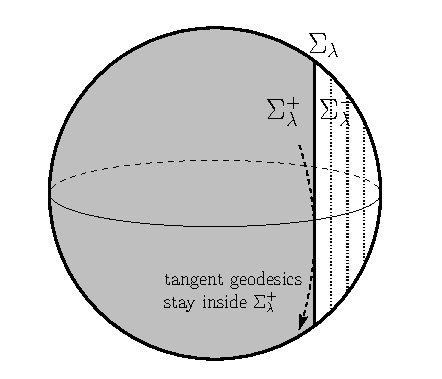
\includegraphics{Figures/ex-foliation-1-legende.pdf} 
\caption{A oriented pseudo-convex foliation without boundary in the sphere $\SS^2$. The surfaces $\Sigma_\lambda$ forms a smooth family of vertical circles inside a hemisphere and $\Sigma_\lambda^+$ and $\Sigma_\lambda^-$ are respectively the large and the small spherical caps. The geodesics beings the great circles, the ones which are tangent to a surface $\Sigma_\lambda$ stay inside~$\Sigma_\lambda^+$.\label{fig-foliation-1}
}
\end{figure}

By a classical argument, we may state a global version of Theorem~\ref{th-hormander} as follows.

\begin{theo}\label{th-hormander-global}
Let $\Omega$ be a smooth compact manifold (with or without boundaries) and let $\omega\subset\Omega$ be an open set. Assume that there exists an oriented pseudo-convex foliation without boundary $(\Sigma_\lambda)_{\lambda\in[0,1)}$ of $\Omega$ in the sense of Definition~\ref{defi-foliation1}. Also assume that $\Sigma_0^+\subset \omega$ and $\omega\cup \left(\bigcup_{\lambda\in[0,1)}
\Sigma_\lambda^+\right)$ covers $\Omega$ up to a set of zero measure.

Let $b$, $c$ and $d$ be bounded coefficients. Assume that $z$ is a global mild solution of
\[
\begin{cases}
\partial^2_{tt} z &=\Delta z + b(x,t)\partial_t z+c(x,t).\grad z+d(x,t)z\quad(x,t)\in\Omega\times \RR\\
z_{|\omega}(x,t)&= 0\mkern297mu(x,t)\in\omega\times\RR
\end{cases}
\]
with any suitable boundary conditions on $\partial\Omega$ such that the wave equation is well-posed and where $\Delta$ is the Laplace--Beltrami operator related to $\Omega$.

Then $z\equiv 0$ everywhere.
\end{theo}


\begin{proof}
We will show that $z(\cdot,t=0)$ vanishes in $\omega\cup\Sigma^+_\lambda$, for all $\lambda\in [0,1)$, which shows that $z(t=0)\equiv 0$ and thus that $z\equiv 0$ due to the uniqueness properties of the wave equation. By assumption, $z\equiv 0$ in $\Sigma_0^+\subset \omega$. Let $\lambda_0\in (0,1)$ and let $h_{\alpha,T}(t)=\alpha(1-t^2/T^2)$. We consider the family of surfaces $t\in [-T,T]\mapsto \Sigma_{h_{\alpha,T}(t)}$ which is locally parametrized by functions $(x,t)\mapsto \psi_{h_{\alpha,T}(t)}(x)$. Notice that it is a smooth family of smooth surfaces since due to Assumption~\eqref{listdef6.4.1} of Definition~\ref{defi-foliation1}. Also notice that the larger is $T$, the smaller are the derivatives of these functions with respect to $t$. By assumption, each function $x\mapsto \psi_\lambda(x)$ is non-characteristic and strongly pseudo-convex as a function independent of $t$. By compactness, there exists $T$ large enough such that $(x,t)\mapsto \psi_{h_{\alpha,T}(t)}(x)$ defines local surfaces which are non-characteristic and pseudo-convex for all $\alpha\in[0,\lambda_0]$ and $t\in[-T,T]$. The parameter $T$ is fixed in the remaining part of the proof and we may omit it in the notations.

Notice that, for any $\alpha$, the family of set $t\in[-T,T]\mapsto
\Sigma^+_{h_\alpha(t)}$ starts inside $\omega$ at $t=-T$ and finishes inside $\omega$ at $t=T$. Moreover, for any small $\alpha$, these sets always stay inside $\omega$ where $z$ vanishes. Assume that there exist $(x,t)$ and $\alpha\in[0,\lambda_0]$ such that $x\in
\Sigma^+_{h_\alpha(t)}$ and $z(x,t)\neq 0$. We set
\begin{equation}\label{eq-demo-global}
\alpha_0=\min\left\{\alpha\in (0,\lambda_0]\,,\,
\exists t\in[-T,T],\exists x\in\Sigma^+_{h_{\alpha}(t)}\text{ such that }z(x,t)\neq 0\right\}\,.
\end{equation}
By continuity, we know that $z(x,t)=0$ for all $x\in
\Sigma^+_{h_{\alpha_0}(t)}$. Moreover, there exists $t_0\in (-T,T)$ and $x_0\in\Sigma_{h_{\alpha_0}(t_0)}$ such that $z$ is not identically zero in any neighborhood of $(x_0,t_0)$. Indeed, otherwise, by compactness, we may extend the set where $z$ vanishes and contradict~\eqref{eq-demo-global}.

To conclude, it remains to use the local unique continuation property of Theorem~\ref{th-hormander} at $(x_0,t_0)$ with the time-space surface defined by $(x,t)\mapsto \psi_{h_{\alpha_0}(t)}(x)$. The continuation implies that $z$ vanishes near $(x_0,t_0)$ which contradicts the construction. Thus, $z(x,t)=0$ for all $t\in [-T,T]$ and $x\in \bigcup_\alpha \Sigma^+_{h_\alpha(t)}$. In particular $z(\cdot,\,t=0)\equiv 0$ in $\bigcup_{\alpha}\Sigma^+_{h_\alpha(0)}=\bigcup_{\lambda\leq\lambda_0}
\Sigma^+_\lambda$. Since these arguments hold for all $\lambda_0<1$ and since $\omega\cup_{\lambda\in [0,1)} \Sigma^+_\lambda$ is $\Omega$ up to a set of measure zero, we have that $z(\cdot,\,t=0)\equiv 0$ in $\Omega$. Well-posedness of the linear wave equation concludes that $z\equiv 0$ everywhere.
\end{proof}


Notice that, as it is stated, this unique continuation result needs an infinite time to be efficient, where Theorem~\ref{th-RZ} only need a finite explicit time. In fact, a careful look to the proof shows that a finite time is sufficient once we know that the family of surface is pseudo-convex and non-characteristic in a uniform way. However, such a bound of convexity is difficult to obtain in general cases and may be even impossible as for the example studied in Section~\ref{section-appli2}.


A typical example of application is given in Figure~\ref{fig-foliation-1}: if $\Omega$ is a sphere and $\omega$ covers more than an hemisphere, then if $z$ is a global solution of a linear wave equation which vanishes in $\omega$ for all times, then $z\equiv 0$. Notice that, in this case, the family of surfaces is uniformly pseudo-convex and the unique continuation holds in fact in finite time even if $z$ is not a global in time solution.



\subsection{Unique continuation through pseudo-convex surfaces with boundary}

The case where the pseudo-convex surfaces $\Sigma_\lambda$ meet the boundary $\partial\Omega$ is more involved. Theorem~\ref{th-hormander} has been generalized to this case by Tataru (see~\cite{Tataru_uniq_analyticCPDE, Tataru, Tataru_uniq_analyticJMPA}). The boundary conditions are more difficult to describe geometrically, so we will only deal here with the case of flat geometry, that is $g(x,\xi)=|\xi|^2$, and the case of Dirichlet boundary condition.

\begin{defi}\label{defi-foliation2}
A family of surfaces $(\Sigma_\lambda)_{\lambda\in[0,1)}$ is an \emph{oriented pseudo-convex foliation with boundary} in a flat manifold $\Omega$ if:
\begin{enumerate}\romanenumi
\item \label{listdef6.6.1}the family of surfaces is smooth in the sense that it is locally described as level sets $\{x,\psi_\lambda(x)=0\}$ where $(x,\lambda)\mapsto\psi_\lambda(x)$ is a local smooth function with $\grad_x\psi_\lambda\neq 0$.
\item \label{listdef6.6.2}each surface is globally oriented in the sense that there exist disjoint sets $\Sigma_\lambda^\pm$ such that locally $\{x\in\Omega,\pm\psi_\lambda(x)> 0\}\subset \Sigma_\lambda^\pm$ and such that $\Omega=\Sigma_\lambda^- \cup
\Sigma_\lambda \cup \Sigma_\lambda^+$.
\item \label{listdef6.6.3}for each $\lambda$, $(x,t)\mapsto \psi_\lambda(x)$ is pseudo-convex in the sense of Definition~\ref{defi-pseudoconvex} as a function independent of $t$. Equivalently, $\Sigma_\lambda^-$ is locally strictly convex in a neighborhood of its boundary: the tangent space to $\Sigma_\lambda$ at $x_0$ is locally included in $\Sigma_\lambda^+$, $x_0$ excepted.
\item \label{listdef6.6.4}if a surface $\Sigma_\lambda$ meet $\partial\Omega$ at $x$, then $\partial_\nu \psi_\lambda(x)<0$. Equivalently, the angle formed by $\Sigma_\lambda$ and $\partial\Omega$ in the region $\Sigma_\lambda^-$ is strictly less than $\pi/2$.
\end{enumerate}
\end{defi}

A typical example of such oriented pseudo-convex foliation with boundary is given in Figure~\ref{fig-foliation-2}. Notice that the condition at the boundary is consistent with the one inside the domain. Indeed, the geodesics are straight lines which bounce at the boundary according to Newton's laws. Geometrically, we ask that any geodesic either crosses $\Sigma_\lambda$ in a transversal way, or stay locally inside $\Sigma_\lambda^+$.
\begin{figure}[ht]
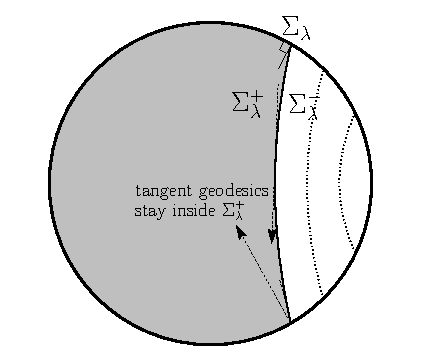
\includegraphics{Figures/ex-foliation-2-legende.pdf} 
\caption{A oriented pseudo-convex foliation with boundary in the disk. The surfaces $\Sigma_\lambda$ forms a smooth family of curves inside a semidisk. The surfaces $\Sigma_\lambda^-$ are strictly convex and the angle formed by $\Sigma_\lambda$ and the boundary of the disk is less than $\pi/2$ on $\Sigma_\lambda^-$ side. The geodesics are straight lines bouncing at the boundary according to Newton's laws. The ones which are tangent to a surface $\Sigma_\lambda$ stay inside $\Sigma_\lambda^+$.\label{fig-foliation-2}
}
\end{figure}

By the same arguments as the ones in the proof of Theorem~\ref{th-hormander-global} and using the result of Tataru, we obtain a global unique continuation result.

\begin{theo}\label{th-hormander-global-2}
Let $\Omega\subset\RR^d$ be a compact domain and let $\omega\subset\Omega$ be an open set. Assume that there exists an oriented pseudo-convex foliation $(\Sigma_\lambda)_{\lambda\in[0,\,1)}$ of $\Omega$ in the sense of Definition~\ref{defi-foliation2}. Also assume that $\Sigma_0^+\subset
\omega$ and $\omega\cup\left(\bigcup_{\lambda\in[0,\,1)} \Sigma_\lambda^+\right)$ covers $\Omega$ up to a set of zero measure.

Let $b$, $c$ and $d$ be bounded coefficients. Assume that $z$ is a global mild solution of
\[
\begin{cases}
\partial^2_{tt}z &=\Delta z + b(x,t)\partial_t z+c(x,t).\grad z+d(x,t)z\quad(x,t)\in\Omega\times \RR\\
z_{|\partial\Omega}(x,t)&=0 \mkern298mu (x,t)\in\partial\Omega\times\RR\\
z_{|\omega}(x,t)&=0 \mkern298mu(x,t)\in\omega\times\RR
\end{cases}
\]
Then $z\equiv 0$ everywhere.
\end{theo}

A typical example of application is given in Figure~\ref{fig-foliation-2}: if $\Omega$ is a disk and $\omega$ covers more than half of the boundary, then if $z$ is a global solution of a linear wave equation which vanishes in $\omega$ for all times, then $z\equiv 0$.

\subsection{Proof of Theorem~\ref{th2}}

Theorem~\ref{th2} is then a direct consequence of the unique continuation results stated in this Section: Proposition~\ref{prop-UCP-implique-th} and Theorems~\ref{th-hormander-global} and~\ref{th-hormander-global-2} imply Theorem~\ref{th2}.



\section{Application 2: the peanut of rotation}\label{section-appli2}

We consider in this section the example of the peanut of rotation: a two-dimensional manifold where a central part is equivalent to the cylinder $\{x=(y,\theta)\in (-1,1)\times\!\SS\!\}$ endowed with the metric $g(y,\theta)=\drm y^2+\cosh^2(y)\drm\theta^2$ (see Figure~\ref{fig-1}). The damping $\gamma$ is assumed to be positive, except in a part $x\in (-\ell,\ell)$ of the central part ($\ell\in (0,1)$). The decay of the linear damped wave semigroup has been established in~\cite{CSVW,Schenck}.

\begin{theo}\label{th-CSVW}
\emph{Christianson, Schenck, Vasy \& Wunsch, 2014.}\\
In the setting of the peanut of rotation, there exist two positive constants $C$ and $\lambda$ such that the semigroup $e^{At}$ satisfies
\[
\left\|e^{At} U_0\right\|_X \leq C e^{-\lambda\sqrt{t}} \|U_0\|_{D(A)}\,.
\]
\end{theo}

The decay rate of Theorem~\ref{th-CSVW} obviously satisfies~\eqref{hyp-decay-1} and~\eqref{hyp-decay-2}. Thus, once the unique continuation property is obtained, Proposition~\ref{prop-UCP-implique-th} yields the conclusion of Theorem~\ref{th1} for the framework of the peanut of rotation. To obtain the unique continuation property, we will apply Theorem~\ref{th-hormander-global} with the family of pseudo-convex surfaces shown in Figure~\ref{fig-foliation-peanut}.

\begin{figure}[ht]
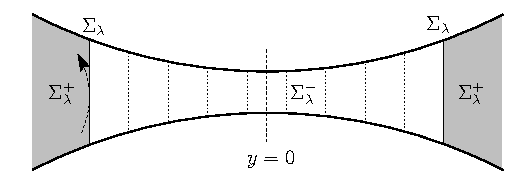
\includegraphics[scale=1.25]{Figures/foliation-peanut-legende.pdf} 
\caption{An oriented pseudo-convex foliation without boundary of the central part of the peanut. Each surface $\Sigma_\lambda$ consists in two vertical circles, the set $\Sigma_\lambda^-$ being the interior part surrounded by these circles. Since the central part of the peanut is negatively curved, the geodesics tangent to the vertical circles stay in the exterior domain $\Sigma_\lambda^+$. Notice that the set $\Sigma_0$ consists in both exterior disk and the disks $\Sigma_\lambda$ get closer to $x=0$ when $\lambda$ get closer to $1$. Thus, the central circle $x=0$ is not included in $\bigcup_{\lambda\in [0,1)}\Sigma_\lambda^+$ but this is not important since this set is of zero measure.\label{fig-foliation-peanut}
}
\end{figure}

Applying Theorem~\ref{th2} and the ideas of Proposition~\ref{prop1}, we obtain the following result.

\begin{theo}\label{th-appli2}
Consider the damped wave equation~\eqref{eq} in the framework of the peanut of rotation introduced above. Let $\alpha>0$ and $f$ satisfying~\eqref{hyp-f-estim} and~\eqref{hyp-f-sign}. Then, any solution $u$ of~\eqref{eq} satisfies
\[
\|(u,\partial_t u)(t)\|_{H^1_0\times L^2}\,\xrightarrow[\:t\longrightarrow
+\infty\:]{}\,0\,.
\]

Moreover, for any $R$ and $\sigma\in (0,1]$, there exists $C_{R,\sigma}$ such that, for any solution $u$ with $U_0\in X^\sigma$,
\[
\|(u_0,u_1)\|_{H^{1+\sigma}\times H^\sigma}\leq
R\:\Longrightarrow\:\|(u,\partial_t u)(t)\|_{H^1_0\times L^2} \leq
C_{R,\sigma}e^{-\sigma\tilde \lambda\sqrt{t}}
\]
where $\tilde\lambda$ is the linearized rate given in Lemma~\ref{lemma-appli2}.
\end{theo}
\begin{proof}
Let us first formally check that the family of disks introduced in Figure~\ref{fig-foliation-peanut} is a suitable pseudo-convex foliation without boundary. We use the cylindrical coordinates $x=(y,\theta)\in (-1,1)\times\SS$ with associated tangent variables $\xi=(\zeta,\Theta)$. By symmetry, we only consider the right-hand-side circles which are defined by $\psi_\lambda(x)=0$ with $\psi_\lambda(x)=y-(1-\lambda)$. The circle $\Sigma_0$ corresponding to $y=1$ is in the interior of the region $\omega$ where the damping is positive. When $\lambda$ get closer to $1$, the circle $\Sigma_\lambda$ get closer to $y=0$. We are obviously in the setting of Definition~\ref{defi-foliation1} and thus of Theorem~\ref{th2}, except maybe for the assumption of strong pseudo-convexity. We already give a geometrical insight of this assumption, but let us check it formally.

The local metric is given by $g(y,\theta)=\drm y^2+\cosh^2(y)\drm\theta^2$. The Laplace--Beltrami operator is thus given by
\[
\Delta_g = \partial_{yy}^2 + 2\tanh(y)\partial_y + \frac 1
{\cosh^2(y)}\partial^2_{\theta\theta}\,.
\]
The principal part of the wave operator is then
\[
p(y,\theta,t,\zeta,\Theta,
\tau)=|\zeta|^2+\frac 1{\cosh^2(y)}|\Theta|^2-|\tau|^2\,.
\]
Thus $H_p(\psi_\lambda)=2\zeta$ and
\[
H_p^2(\psi_\lambda)=4 \frac{\sinh(y)}{\cosh(y)^3} |\Theta|^2\,.
\]
The pseudo-convexity condition is then checked. Indeed, if $H_p(\psi_\lambda)=0$ then $\zeta=0$ and since $\xi=(\zeta,\Theta)$ must be non-zero, we must have $\Theta\neq 0$. As $\psi_\lambda(y,\theta)=0$ with $\lambda\in[0,1)$, we have $y>0$ and thus $H_p^2(\psi_\lambda)>0$. Looking carefully to the computations, one notes that, in fact, we only need that the radius $\cosh(y)$ of the cylindrical part is increasing for $y>0$ and decreasing for $y<0$ to obtain the unique continuation property.

The above arguments show the stabilization of the semilinear damped wave equation. Moreover, Proposition~\ref{prop-asymp-compact-2} shows the uniform convergence to $0$ in $X^{\sigma'}$ for initial data in a more regular space $X^\sigma$ ($\sigma>\sigma'$).

To obtain the decay estimate of Theorem~\ref{th-appli2}, we argue as in the proof of the second case of Proposition~\ref{prop1}. However, we claim that we can avoid the loss in the power by following Remark~\ref{remark-log}. Indeed, \cite[Theorem~5.1]{CSVW} implies in our framework that, for large $\mu$,
\[
\left\|(-\Delta+\mu^2-i\mu\gamma)^{-1}\right\|_{\Lc(L^2)}\,\leq\,
C\,\frac{\ln|\mu|}{|\mu|}\,.
\]
We argue as in the proof of Lemma~\ref{lemma-appli2}. Applying Propositions~\ref{prop-resolvent}, \ref{prop-estimP} and~\ref{prop-appendix-linearized}, we obtain
\[
\left\|(\tilde A-i\mu)^{-1}\right\|_{\Lc(L^2)} \leq C \, {|\ln \mu|}\,.
\]
and by Theorem~\ref{th-BD}, we get the conclusion of Lemma~\ref{lemma-appli2} in the form
\[
\left\|e^{\tilde A t}U_0\right\|_X \leq Ce^{-b\sqrt{t}} \|U_0\|_{D(A)}\,.
\]
In other words, we avoid an additional logarithmic loss by directly dealing with the estimates of~\cite{CSVW} instead of using the back and forth implications of Theorems~\ref{th-BD-1} and~\ref{th-BD}.

It is then sufficient to follow the proof of the exponential case of Proposition~\ref{prop1} with the exponent $\gamma=1/2$.
\end{proof}


\section{Decay estimate in the disk with holes}\label{section-decay-disk}
In the previous examples of application, the decay of the semigroups was explicitly written in previous papers. In the case of a disk with several holes, we are not aware of a paper where an explicit decay is written. The corresponding scattering problem has been studied by Ikawa in~\cite{Ikawa1,Ikawa2}. Many further studies have been published. In this article, we will use an estimate and a ``black box argument'' introduced by Burq and Zworski in~\cite{Burq-Zworski}. Combining them with the results in Appendix, we obtain the following decay.

\begin{theo}\label{th-decay-disque-trous}
Let $\Oc\subset\RR^d$ be a smooth bounded open set. For $i=1\ldots p$, let $O_i\subset \Oc$ be smooth strictly convex obstacles satisfying:
\begin{enumerate}\alphenumi
\item \label{listtheo8.1.1}the obstacles are disjoint: $O_i\cap O_j=\emptyset$ for $i\neq j$,
\item \label{listtheo8.1.2}the convex hull $\cnvh(\cup_i O_i)$ of the obstacles is contained in $\Oc$,
\item \label{listtheo8.1.3}no obstacle is in the convex hull of two others, that is that $\cnvh(O_i\cup O_j)\cap O_k =\emptyset$ for $i,j,k$ different,
\item \label{listtheo8.1.4}if there are three or more obstacles ($p>2$), set $\kappa$ the infimum of the principal curvatures of the boundaries $\partial O_i$ of the obstacles and $L$ the minimal distance between two obstacles, and assume that $\kappa L>p$.
\end{enumerate}
Let $O=\cup_i O_i$, let $\Omega=\Oc\setminus O$ be the domain with holes and let $\gamma\geq 0$ be a damping which is strictly positive in a neighborhood of the exterior boundary $\partial \Oc$. Then the semigroup $e^{At}$ of the linear damped wave equation on $\Omega$ satisfies
\[
\left\|e^{At}U_0\right\|_X \leq C e^{-\lambda t^{1/3}} \|U_0\|_{D(A)}
\]
with $C$ and $\lambda$ two positive constants.
\end{theo}

A typical domain consists in a smooth domain with several small holes as in Figure~\ref{fig-disque-trous}. Typically, if $O_i$ are balls of center $c_i$ and radius $r_i$ and if there is no triplet of aligned centers, then Assumption~\eqref{listtheo8.1.4} holds for $r_i$ small enough since $\kappa$ becomes large whereas $L$ stay bounded.

\begin{figure}[ht]

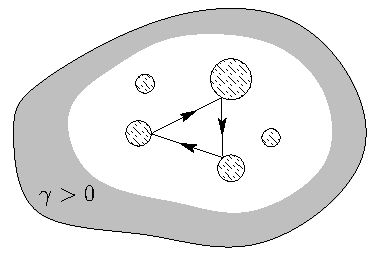
\includegraphics[scale=1]{Figures/disque-trous-2-legende.pdf} 

\caption{A domain satisfying Hypotheses~\eqref{listtheo8.1.1}-\eqref{listtheo8.1.4} of Theorem~\ref{th-decay-disque-trous}. Notice the presence of periodic geodesics bouncing on the obstacles and never meeting the support of the damping $\gamma$. The geometric control condition thus fails and we cannot hope a uniform decay of the semigroup in $X$. \label{fig-disque-trous}}
\end{figure}

\goodbreak
\begin{remas}\ \\*[-1.4em]
\begin{itemize}
\item We do not claim that the decay rate $e^{-t^{1/3}}$ is optimal. In fact, our proof uses rough arguments leading to logarithmic losses. We strongly believe that the right decay rate is $e^{-t^{1/2}}$. A strategy of proof may be to follow the arguments of Datchev and Vasy~\cite{Vasy}, adding the presence of a boundary. However, this improvement is not central and would use techniques too far from the spirit of this paper.
\item It is also certainly possible to relax the assumption about $\gamma$ to the following weaker assumption. There exists a neighborhood $K$ of $O=\cup_i O_i$ such that any geodesic ray starting in $\Omega\setminus K$ reach a point where $\gamma\geq \varepsilon >0$ before meeting $K$, for at least the backward or the forward flow.
\end{itemize}
\end{remas}

Based on~\cite{Ikawa2}, the following estimate appears in~\cite{Burq-Zworski}

\begin{prop}\label{prop-BZ}
\emph{Ikawa's black box (\cite[Section~6.2]{Burq-Zworski})}
Let $O_i$ be obstacles in $\RR^d$ satisfying the Assumptions~\eqref{listtheo8.1.1}, \eqref{listtheo8.1.3} and~\eqref{listtheo8.1.4} of Theorem~\ref{th-decay-disque-trous}. Let $R_{bb}(\mu)$ be the outgoing resolvent of the Laplacian operator outside the obstacles, that is the meromorphic continuation of $(\Delta_{\RR^d\setminus O}+\mu^2)^{-1}$ from Im$(\mu)>0$, where $\Delta_{\RR^d\setminus O}$ is the Laplacian operator on the exterior domain ${\RR^d\setminus O}=\RR^d\setminus (\cup_i O_i)$ with Dirichlet boundary condition.

Then, for any cut-off function $\chi\in\Cc^\infty_c(\RR^d)$, we have
\[
\|\chi R_{bb}(\mu) \chi\|_{\Lc\left(L^2({\RR^d\setminus
O})\right)} \leq C \frac {\ln (1+|\mu|)}{1+|\mu|}\,.
\]
\end{prop}

Using this black box in the same spirit of~\cite{Burq-Zworski}, we obtain the following observation estimate.

\begin{lemm}\label{lemma-BZ}
Assume that the assumptions of Theorem~\ref{th-decay-disque-trous} hold. Then there exists $C>0$ such that
\[
\forall \mu\in\RR\,,\:\forall u\in D(\Delta)\,,\:\|u\|_{L^2(\Omega)}\,\leq\,
C\frac {\ln |\mu|}{|\mu|} \|(\Delta+\mu^2)u\|_{L^2(\Omega)} + C{\ln |\mu|}\:
\|\sqrt{\gamma} u \|_{L^2(\Omega)}
\]
where $\Delta$ is the Laplacian operator on the bounded domain with holes $\Omega=\Oc\setminus O$ with Dirichlet boundary conditions.
\end{lemm}
\begin{proof}
By compactness, there exists $\varepsilon>0$ such that $\gamma\geq \varepsilon >0$ in a neighborhood of the exterior boundary $\partial \Oc$. Let $\chi\in\Cc^\infty_0(\RR^d)$ be a smooth cut-off function equal to $1$ in a neighborhood of \emph{convhull}$(\cup_i O_i)$, equal to $0$ outside $\Oc$ and such that $1-\chi$ is supported where $\gamma\geq \varepsilon >0$. This is possible by Assumption~\eqref{listtheo8.1.2}. We have immediately
\begin{equation}\label{eq-lemma-BZ-1}
\forall u\in L^2(\Omega)\,,\:\|(1-\chi) u\|_{L^2(\Omega)} \leq \frac 1{\sqrt{\varepsilon}} \|\sqrt{\gamma} u\|_{L^2(\Omega)}\,.
\end{equation}
Let $\chi_0$ be a smooth cut-off function supported in $\Omega$ so that $\chi_0\equiv 1$ in a neighborhood of the support of $\chi$ and let $\chi_1$ be another smooth cut-off function supported in $\Omega$ so that $\chi_1\equiv 1$ in a neighborhood of the support of $\chi_0$. For all $u\in H^2(\Omega)\cap H^1_0(\Omega)$, we extend $\chi_i u$ as a function in $H^2(\RR^d\setminus O)\cap H^1_0(\Omega)$. Regarding $\chi_i u$, applying $\Delta_{\RR^d\setminus O}$ or $\Delta$ gives the same result. We can thus apply the ``black box'' estimate of Proposition~\ref{prop-BZ} as follows.
\begin{align*}
\|\chi u\|_{L^2(\Omega)} & = \left\|\chi \chi_0^2 u\right\|_{L^2(\Omega)} = \left\|\chi\chi_0 R_{bb}(\mu)\left(\Delta+\mu^2\right)\chi_0 u\right\|_{L^2(\Omega)}\\
&\leq \left\|\chi\chi_0 R_{bb}(\mu)\chi_0\left(\Delta+\mu^2\right) u\right\|_{L^2(\Omega)} + \left\|\chi\chi_0 R_{bb}(\mu) [\Delta,\chi_0] u\right\|_{L^2(\Omega)}\\
&\leq \|\chi_0 R_{bb}(\mu)\chi_0\|_{\Lc\left(L^2(\RR^d\setminus O)\right)}
\|\left(\Delta+\mu^2\right)u\| \\
&\mkern200mu+ \left\|\chi\chi_0\chi_1 R_{bb}(\mu)\chi_1 \left[\left(\Delta+\mu^2\right),\chi_0\right] u\right\|\\
&\leq \|\chi_0 R_{bb}(\mu)\chi_0\|_{\Lc\left(L^2(\RR^d\setminus O)\right)}\|\left(\Delta+\mu^2\right) u\|\\
&\mkern200mu + \left\|\chi_1 R_{bb}(\mu)\chi_1\right\|_{\Lc\left(L^2(\RR^d\setminus O)\right)}
\|[\Delta,\chi_0] u\|\\
&\leq C \frac {\ln (1+|\mu|)}{1+|\mu|}\left(\left\|\left(\Delta+\mu^2\right) u\right\|_{L^2(\Omega)} + \|u\|_{H^1(\text{supp}(\grad \chi_0))}\right)\,.
\end{align*}
By interpolation and elliptic regularity, we have
\begin{align*}
\|u\|^2_{H^1(\text{supp}(\grad \chi_0))} & \leq C \|u\|_{L^2(\text{supp}(\grad
\chi_0))} \|u\|_{H^2(\text{supp}(\grad \chi_0))}\\
&\leq C \|u\|_{L^2(\text{supp}(\grad \chi_0))}\left(\|\Delta u\|_{L^2(\text{supp}(\grad \chi_0))} + \|u\|_{L^2(\text{supp}(\grad
\chi_0))}\right)\\
&\leq C \|u\|_{L^2(\text{supp}(\grad
\chi_0))}\left(\|(\Delta+\mu^2)u\|_{L^2(\text{supp}(\grad \chi_0))}\right.\\
& \mkern305mu + \left.\left(1+\mu^2\right)\|u\|_{L^2(\text{supp}(\grad \chi_0))}\right)\\
& \leq\!C\!\left(\!\frac 1{2(1+\mu^2)}\|\!\left(\Delta+\mu^2\right)u\|_{L^2(\text{supp}(\grad
\chi_0))}\! +\!
\frac 32\!\left(1+\mu^2\right)\!\!\|u\|_{L^2(\text{supp}(\grad \chi_0))}\!\right)
\end{align*}
Since the support of $\grad\chi_0$ is included in the place where $\gamma\geq
\varepsilon >0$, both previous estimates yield
\[
\|\chi u\|_{L^2(\Omega)} \leq C \frac {\ln (1+|\mu|)}{1+|\mu|}\left(
\|\left(\Delta+\mu^2\right) u\|_{L^2(\Omega)}
+ (1+|\mu|)\|\sqrt \gamma u\|_{L^2(\Omega)}\right)\,.
\]
With~\eqref{eq-lemma-BZ-1}, this concludes the proof.
\end{proof}

\begin{proof}[{Proof of Theorem~\ref{th-decay-disque-trous}.}] Applying Propositions~\ref{prop-1-appendix} and~\ref{prop-estimP} in Appendix, the observability estimate of Lemma~\ref{lemma-BZ} implies that there exists $C>0$ such that
\[
\forall \mu\in\RR\,,\:\|(A-i\mu)\|_{\Lc(X)}\,\leq\,C \ln^2(2+|\mu|)\,.
\]
Then, we apply Theorem~\ref{th-BD} of Batty and Duyckaerts stated in Appendix to obtain the decay with rate $e^{-\lambda t^{1/3}}$. Notice that Proposition~\ref{prop-1-appendix} and Theorem~\ref{th-BD} contain some losses transforming the rate $\ln |\mu|$ of Lemma~\ref{lemma-BZ} into first $\ln^2 |\mu|$ and then $\ln^3 |\mu|$. This is responsible of the power $1/3$ in the decay rate.
\end{proof}



\section{Application 3: the disk with two holes}\label{section-appli3}

In the previous section, we have obtained a sufficiently fast decay rate for the semigroup of the damped wave equation in a disk with several holes as in Figure~\ref{fig-1}. If we prove the unique continuation property of Proposition~\ref{prop-UCP-implique-th} in this situation, then we would obtain the desired stabilization. To obtain the unique continuation property, we would like to use Theorem~\ref{th-hormander-global-2}, that is to exhibit an oriented pseudo-convex foliation $(\Sigma_\lambda)_{\lambda\in[0,1)}$ with $\Sigma^+_0$ included in a neighborhood of the boundary and $\cup_\lambda \Sigma^+\infty$ covering almost all $\Omega$. This is possible in the case where there is at most two holes in the disk and impossible if there are more holes, as shown in Figure~\ref{fig-appli3}.

\begin{figure}[ht]
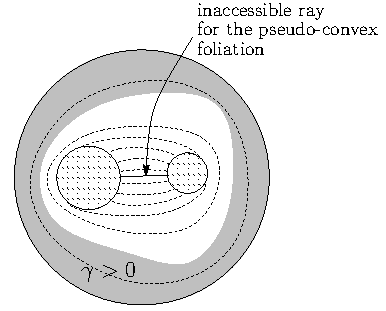
\includegraphics{Figures/disque-trous-3-legende.pdf}\quad 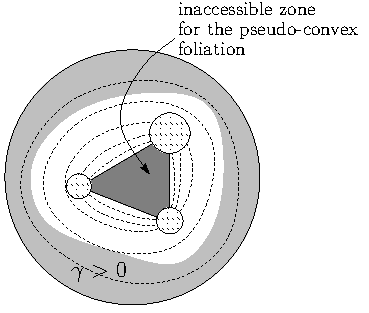
\includegraphics{Figures/disque-trous-4-legende.pdf} 
\caption{Two examples of disks with holes and associated attempts to draw a suitable pseudo-convex foliation covering the whole domain. Left, the disk with two holes may be covered by a pseudo-convex foliation starting in a neighborhood of the exterior boundary, except for a single line, which is of measure zero. Right, an attempt to cover a disk with three holes with a pseudo-convex foliation. We easily notice that the central zone cannot be covered and Theorem~\ref{th-hormander-global-2} cannot be applied in this case.}\label{fig-appli3}
\end{figure}

Thus, in the case where there is only two holes, Theorem~\ref{th-hormander-global-2} enables to use Proposition~\ref{prop-UCP-implique-th} and to obtain the conclusions of Theorem~\ref{th1}. Moreover, notice that in this case, there is no technical assumptions, neither~\eqref{listtheo8.1.3} nor~\eqref{listtheo8.1.4}, in Theorem~\ref{th-decay-disque-trous}. We thus obtain the following result, as an application of Theorem~\ref{th2}, Proposition~\ref{prop1} and mutatis mutandis the same use of Remark~\ref{remark-log} as in the proof Theorem~\ref{th-appli2}. The proof is left to the reader.

\begin{theo}\label{th-appli3}
Consider the damped wave equation~\eqref{eq} in the framework of a disk with two convex holes and assume that the damping $\gamma$ is strictly positive in a neighborhood of the exterior boundary. Let $\alpha>0$ and $f$ satisfying~\eqref{hyp-f-estim} and~\eqref{hyp-f-sign}. Then, any solution $u$ of~\eqref{eq} satisfies
\[
\|(u,\partial_t u)(t)\|_{H^1_0\times L^2}\,\xrightarrow[\:t\longrightarrow
+\infty\:]{}\,0\,.
\]

Moreover, there exists $\tilde\lambda$ such that, for any $R$ and $\sigma\in (0,1]$, there exists $C_{R,\sigma}$ such that, for any solution $u$ with $U_0\in X^\sigma$,
\[
\|(u_0,u_1)\|_{H^{1+\sigma}\times H^\sigma}\leq
R\:\Longrightarrow\:\|(u,\partial_t u)(t)\|_{H^1_0\times L^2} \leq
C_{R,\sigma}e^{-\sigma\tilde \lambda{t}^{1/3}}\,.
\]
\end{theo}


\section{Analytic regularization and proof of Theorem~\ref{th1}}\label{section-reg-analytic}

In Figure~\ref{fig-appli3}, we have seen that, in some situations, the unique continuation property of Lerner--Robbiano--H\"ormander stated in Theorem~\ref{th-hormander-global-2} is not useful. To deal with these situations, we need another unique continuation property: Theorem~\ref{th-RZ} of Robbiano--Zuily--H\"ormander to~\eqref{eq-UCP}. This is only possible if the coefficients of~\eqref{eq-UCP} are analytic with respect to the time $t$. Thus, we need to choose $f'_u$ analytic with respect to $u$ and to prove that the global solution $w$ appearing in~\eqref{eq-UCP} is analytic in time. This is the basic idea leading to Theorem~\ref{th1}.

However, even if $f$ is analytic, the damped wave equation does not regularize its solutions. To overcome this problem, we use the following fact known since the work of Hale and Raugel in~\cite{Hale-Raugel}: the globally bounded solutions of the damped wave equation are as smooth as the non-linearity $f$. This asymptotic regularization property is linked to the asymptotic smoothness or compactness property (see Section~\ref{section-asymp-compact}). The idea that this asymptotic smoothing of the damped wave equation may be used to apply analytic unique continuation theorems originates from the work of Hale and Raugel, even if they did not publish this idea. The first published occurrence appears in~\cite{RJ} (see also~\cite{RC}).

The article~\cite{Hale-Raugel} contains several abstract theorems. They apply for linear semigroup with uniform decay, that is $\|e^{At}\|_{\Lc(X)}\leq M e^{-\lambda t}$. The purpose of the present article is to study cases where this uniform decay fails, so~\cite{Hale-Raugel} does not directly apply: we need to extend its results in our case where the semigroup has a weaker decay. Extending these results in the most general framework will lead to heavy notations and assumptions. That is why, we only consider here damped wave equations in a simple setting and in low dimension.

\subsection{Analytic regularization of global bounded solutions}
Let $d=2$ or $3$ and let $\Omega$ be a smooth manifold of dimension $d$ with or without boundary and such that $\overline\Omega$ is compact. Let $\gamma\in \Cc^1(\Omega,\RR)$ be a nonnegative damping, let $\Delta$ be the Laplacian operator with Dirichlet boundary condition and let $f\in\Cc^\infty(\overline\Omega\times\RR,\RR)$ be a smooth nonlinearity. We assume that $f$ is of polynomial type in the sense that there exist $p>0$ and $C>0$ such that~\eqref{hyp-f-estim} holds. We consider global solutions of the damped wave equation
\begin{equation}\label{eq-analytic}
\begin{cases}
\partial_{tt}^2 u(x,t) + \gamma(x)\partial_t u(x,t) &= \Delta u(x,t) - \alpha u(x,t)\\
& \mkern 85mu - f(x,u(x,t))\quad\,(x,t)\quad\in\;\;\Omega\times \RR\\
\mkern117mu u_{|\partial\Omega}(x,t)&= 0\;\mkern177mu(x,t)\quad\in\partial\Omega\times \RR
\end{cases}
\end{equation}

We use the notations of Section~\ref{section-basic}. In particular, for $\sigma\in[0,1]$, we set\linebreak$X^{\sigma}=(H^{1+\sigma}(\Omega)\cap H^1_0(\Omega))\times H^{\sigma}_0(\Omega)$, $X^0=X=H^1_0(\Omega)\times L^2(\Omega)$ and $X^1=D(A)$. Also notice that $H^{1+\sigma}(\Omega)$ is a subspace of $\Cc^0(\overline\Omega)$ for $d=2$ and $\sigma>0$ or for $d=3$ and $\sigma>1/2$.

The purpose of this section is to prove the following result

\begin{theo}\label{th-analytic}
Assume that the above setting holds, in particular assume that $\gamma\in \Cc^1(\Omega,\RR)$. Let $U(t)\in\Cc^0(\RR,X)$ be a mild solution of~\eqref{eq-analytic} and assume moreover that
\begin{enumerate}\romanenumi
\item \label{listtheo10.1.1}There exists $\sigma_0\in (0,1)$ such that $U(t)$ is defined for all $t\in\RR$ and uniformly bounded in $X^{\sigma_0}$, that is that there exists $C>0$ such that
\[
\forall t\in\RR\,,\:\|U(t)\|_{X^{\sigma_0}}\leq C\,.
\]
If $d=3$, assume in addition that $\sigma_0>1/2$.
\item \label{listtheo10.1.2}The linear semigroup satisfies the decay estimate
\begin{equation}\label{hyp-decay-analytic}
\forall U_0\in D(A)\,,\,\left\|e^{At}U_0\right\|_X\,\leq\,\frac M {t^{\beta}}\,\|U_0\|_{D(A)}
\end{equation}
with $\beta>\max(2p,2/(1-\sigma_0))$, where $p$ is the polynomial growth of $f$ in~\eqref{hyp-f-estim}.
\item \label{listtheo10.1.3}The function $u\in\RR \mapsto f(x,u)\in\RR$ is analytic with respect to $u$,
\end{enumerate}
Then the mapping $t\in\RR \mapsto U(t)\in X^{\sigma_0}$ is analytic with respect to $t$.
\end{theo}

We expect that the condition $\beta>2p$ in Assumption~\eqref{listtheo10.1.2} is not optimal: at least $\beta>p$ should be sufficient if we get rid of the losses in the too general proofs of the auxiliary results in appendix and $\beta>2/(1-\sigma_0)$ could be omitted by assuming more regularity on $\gamma$. Since our concrete applications have a linear decay of the type $\Oc(e^{-t^{\beta}})$, we let these probable improvements for later study.

%\vspace{3mm}

The remaining part of this section is devoted to the proof of Theorem~\ref{th-analytic}.
\begin{proof}[{Proof of Theorem~\ref{th-analytic}}]

%{\noindent $\bullet$ Step 1:
\begin{step}\emph{A trick to satisfy the boundary condition.\label{step1prooftheo10.1}}
 
We would like that $u\mapsto f(\cdot,u)$ maps $H^{1+\sigma}(\Omega)\cap H^1_0(\Omega)$ into $H^\sigma_0(\Omega)$. For $d=2$ or $d=3$ and $\sigma>1/2$, the regularity part is trivial since $H^{1+\sigma}(\Omega)\subset \Cc^0(\Omega)$ is a normed algebra. However, the boundary condition is not necessarily fulfilled since $f(x,0)$ may be different from $0$. Let us describe here a trick introduced in~\cite{Hale-Raugel} to deal with this problem. Let $e$ be the (time-independent) solution of $\Delta e -\alpha e = f(x,0)$ in $H^2(\Omega)\cap H^1_0(\Omega)$. We notice that $\tilde u=u-e$ solves
\[
\partial^2_{tt} \tilde u + \gamma(x)\partial_t \tilde u = \Delta \tilde u -
\alpha \tilde u - f(x,\tilde u + e(x)) + f(x,0)\,.
\]
If we set
\[
\tilde f(x,\tilde u)= f(x,\tilde u + e(x)) - f(x,0)
\]
we obtain a function $\tilde f$ as smooth as $f$ which is also analytic with respect to $\tilde u$. Moreover, $\tilde f(x,0)=0$ for $x\in\partial\Omega$, which shows that $\tilde u\mapsto \tilde f(\cdot,\tilde u)$ maps $H^{1+\sigma}(\Omega)\cap H^1_0(\Omega)$ into $H^\sigma_0(\Omega)$, including the boundary condition. If we prove Theorem~\ref{th-analytic} for $\tilde u$ and $\tilde f$, it clearly yields Theorem~\ref{th-analytic} for $u$ and $f$. Thus, we may assume that $f(x,0)=0$ at the boundary and we will forget the tilde sign to lighten the notations in what follows. In particular, $F=(0,f)$ maps $X^\sigma$ into $X^{1+\sigma}$.
\end{step}

%\vspace{3mm}

\begin{step}\emph{The decay of the high-frequencies semigroups\label{step2prooftheo10.1}}

From now on, we also use the notations of the appendices, Sections~\ref{section-appendix1} and~\ref{section-appendix2}. In particular, we set $L=-\Delta+\alpha$. Since $L$ is self-adjoint, positive and with compact resolvent, there exists an orthonormal basis $(\phi_k)_{k\geq 0}$ of eigenfunctions of $L$ corresponding to the eigenvalues $(\lambda_k)_{k\geq 0}$. As in Section~\ref{section-appendix2}, we introduce the high-frequencies truncations $Q_n$, that are the projectors on the space span$\{\phi_k,k\geq n\}$ and we set $\Qc_n=(Q_n,Q_n)$ on $X$.

The proof of Theorem~\ref{th-analytic} is based on the following splitting. We introduce $P_n=Id-Q_n$ and $\Pc_n=Id-\Qc_n$, which are low-frequencies projections with finite rank. We consider the splitting
\begin{equation}\label{eq-proj2}
U\,=\,\Pc_n U + \Qc_n U\,:=\,V+W\,.
\end{equation}
Then~\eqref{eq-analytic} writes
\begin{equation}\label{eq-proj}
\begin{cases}
\partial_t V &= (\Pc_nA\Pc_n) V +
(\Pc_nA\Qc_n)W+\Pc_n F(V+W)\\
\partial_t W &= (\Qc_nA\Qc_n) W + (\Qc_nA\Pc_n)V+\Qc_n F(V+W)\\
\end{cases}
\end{equation}


As a consequence of the results in the appendices, we have the following decay estimates.

\begin{prop}\label{prop-ana-1}
Assume that Hypothesis~\eqref{listtheo10.1.2} of Theorem~\ref{th-analytic} holds. Then, for all $\sigma\in[0,1)$, $\nu\in (0,1-\sigma]$ and $\varepsilon>0$, there exists $C>0$ such that, for all $n\in\NN$,
\begin{equation}\label{eq-th-decay-2}
\forall t\geq 0\,,\,\forall U\in \Qc_n X^{\sigma+\nu}\:\left\|e^{\Qc_nA\Qc_n t} U\right\|_{X^\sigma}\,\leq\,\frac C {t^{\nu
\beta/2-\varepsilon}} \, \|U\|_{X^{\sigma+\nu}}\,.
\end{equation}
\end{prop}
\begin{proof}
Using the arguments of Proposition~\ref{prop-decay-interpole}, it is sufficient to obtain the decay for $\sigma=0$ and $\nu=1$, that is the decay estimate from $D(A)$ into $X$.

In the appendices, we recall the result of Borichev and Tomilov in~\cite{Bor-Tom} (see Theorem~\ref{th-BT}). In the context of the damped wave equation, we may also consider~\cite[Proposition~2.4]{Ana-Leau} by Anantharaman and Léautaud. We obtain that Hypothesis~\eqref{listtheo10.1.2} of Theorem~\ref{th-analytic} implies the estimate
\begin{equation}
\|u\|_{L^2}\leq C \left(|\mu|^{1/\beta-1} \|P_B(\mu)u\|_{L^2} + |\mu|^{1/2\beta} \left\|\sqrt{B} u \right\| \right)
\end{equation}
with $B$ is the multiplication by $\gamma$ and $P_B(\mu)=-L-i\mu B+\mu^2 Id$. Note that the unique continuation assumed in~\cite[Proposition~2.4]{Ana-Leau} is satisfied because Hypothesis~\eqref{listtheo10.1.2} is satisfied. Thus, we obtain that
\begin{equation}\label{eq-demo-analytic-1}
\|u\|_{L^2}\leq C \left(|\mu|^{1/\beta-1} \|P(\mu)u\|_{L^2} +
\left(|\mu|^{1/\beta} \left\|\sqrt{B}\right\|_{\Lc(L^2)} + |\mu|^{1/2\beta}\right)
\left\|\sqrt{B} u\right\| \right)
\end{equation}
with $P(\mu)=-L+\mu^2 Id$. Then, Propositions~\ref{prop-1-appendix-high-frequencies} and~\ref{prop-2-appendix} show that
\[
\forall n\in\NN\,,\:\forall \mu\in\RR\,,\:\left\|(\Qc_n A \Qc_n -
i\mu)^{-1}\right\|_{\Lc(\Qc_n X)}\,\leq\,\frac K{|\mu|^b}
\]
with $b=2/\beta$. At this point, we may use Theorem~\ref{th-BT} in appendix to obtain the decay of the linear semigroup. However, this result of~\cite{Bor-Tom} (as the one of~\cite{Ana-Leau}) is not stated with explicit constants and we need to be sure that these constants are uniform in $n$ (even if this is surely the case). Thus, we accept here a small loss (harmless for the proof of Theorem~\ref{th-analytic}) and we use the explicit statement of Theorem~\ref{th-BD} to obtain that, for any $\varepsilon>0$, there exists a constant $C$ such that
\[
\left\|e^{\Qc_nA\Qc_n t} U\right\|_{X}\,\leq\,\frac C
{t^{\beta/2-\varepsilon}}
\, \|U\|_{D(A)}
\]
which concludes the proof.
\end{proof}
\end{step}

%\vspace{3mm}
%%step3
\begin{step}\emph{The finite determining modes\label{step3prooftheo10.1}}

In this step, we follow the arguments of~\cite{Hale-Raugel} with the main modifications coming from the weaker decay of the linear semigroup. We consider the complex setting, that is that the functions in $X$ are complex valued. We recall that a function $\Psi$ between two complex Banach spaces $Y$ and $Z$ is said to be holomorphic if its Fréchet derivative exists for any $y\in Y$. We introduce the notation
\[
\Bc_{M,\delta}(Y) = \left\{U(t)\in \Cc^0(\RR,Y)\:|\:\forall
t\in\RR,\,\|\Re(U(t))\|_Y\leq M\text{ and }\|\Im(U(t)\|_Y \leq \delta \right\}\,.
\]
The space $\Bc_{M,\delta}(Y)$ is naturally endowed with the $L^\infty(Y)$-norm. We assumed that $\sigma_0>0$ for $d=2$ and $\sigma_0>1/2$ for $d=3$ as in Hypothesis~\eqref{listtheo10.1.3} of Theorem~\ref{th-analytic}, so that $H^{1+\sigma_0}(\Omega)\subset \Cc^0(\Omega)$.

We will use the holomorphic extension of $f$ in a technical setting stated in the following Lemma~\ref{lemm10.3}. Except this particular setting, the result is a straightforward consequence of the analyticity of $f$ and we omit the proof.
\begin{lemm}\label{lemm10.3}
Assume $u\in\RR \mapsto f(x,u)\in\RR$ is analytic with respect to $u$. Denote $\kappa$ the injection constant $\|\cdot\|_{L^\infty}\leq \kappa
\|\cdot\|_{H^{1+\sigma_0}}$.

Let $M$ be given and $M'_0\geq 0$. Then, there exists $M'\geq M'_0$, as well as two small positive constants $\delta$ and $\delta'$ such that the following holds. The function $z\in\RR \mapsto f(\cdot,z)\in \Cc^1(\overline\Omega,\RR)$ has a holomorphic extension in 
\[
\big\{z\in\CC,\,|\Re(z)|\leq \kappa(M+M'+\delta)\text{ and }|\Im(z)|\leq \kappa(\delta+\delta')\big\}\,.
\]
\end{lemm}

We apply the above Lemma~\ref{lemm10.3} to obtain the following result.

\begin{prop}\label{prop-W}
Let $M$ and $M'_0\geq 0$ be given and let $n_0\in\NN$. Let $M'$, $\delta$ and $\delta'$ the constants given by the previous Lemma~\ref{lemm10.3}. Then, there exist $n\geq n_0$ so that for any function $V(t)$ in the complex set $\Bc_{M+\delta,\delta}(\Pc_nX^{\sigma_0})$, there exists a unique bounded solution $W$ in $\Bc_{M',\delta'}(\Qc_nX^{\sigma_0})$ of
\begin{equation}\label{eq-prop-W}
\partial_t W = (\Qc_nA\Qc_n) W + (\Qc_nA\Pc_n) V+\Qc_n F(V+W)\,.
\end{equation}
In addition, the mapping $V\mapsto W(V)$ is lipschitzian and holomorphic.
\end{prop}
\begin{proof}
Assume that $W$ solution of~\eqref{eq-prop-W} exists and is bounded in $\Cc^0(\RR,\Qc_nX^{\sigma_0})$. Then,
\begin{align*}
W(t)=&e^{\Qc_n A\Qc_n (t-t_0)}W(t_0) \\
&\:+\,\int_{0}^{t-t_0} e^{\Qc_n A\Qc_n s}\big((\Qc_nA\Pc_n) V(t-s)+\Qc_n F(V+W)(t-s)\big)\,\drm s.
\end{align*}
Using Proposition~\ref{prop-ana-1}, when $t_0$ goes to $-\infty$, we get
\[
W(t)= \int_{0}^\infty e^{\Qc_n A\Qc_n s}\big((\Qc_nA\Pc_n)
V(t-s)+\Qc_n F(V+W)(t-s)\big)\,\drm s\,.
\]
Conversely, it is easy to see that a solution of the previous integral equation is a solution of~\eqref{eq-prop-W}. To prove Proposition~\ref{prop-W}, we set up a fixed point theorem for contracting maps. We introduce the map $\Phi_{V}$, defined for $W$ bounded in $\Cc^0(\RR,\Qc_nX^{\sigma_0})$~by
\[
\Phi_{V}(W)(t)=\int_0^\infty e^{\Qc_n A\Qc_n
s}\big((\Qc_nA\Pc_n)V(t-s)+\Qc_n F(V+W)(t-s)\big)\,\drm s\,.
\]

During the first part of the proof, we consider real valued functions, so that the terms including the function $f$ are well defined. Let $\nu\in (0,1-\sigma_0]$ to be fixed later. Let $V=(v_1,v_2)$, we have $\Qc_n A\Pc_n V= (0,Q_n\gamma(x)P_n v_2)$. Thus, using that $\gamma$ is of class~$\Cc^1$,
\[
\|\Qc_n A \Pc_n V\|_{X^{\nu+\sigma_0}} \leq C \|P_n
v_2\|_{H^{\nu+\sigma_0}} \leq C |\lambda_n|^{\nu/2}\|P_n
v_2\|_{H^{\sigma_0}}
\]
where $(-\lambda_k)$ denotes the eigenvalues of the Laplacian operator $L$. Proposition~\ref{prop-ana-1} and the bound on $V$ show that
\begin{equation}\label{eq-demo-prop-W-1}
\left\| \int_0^\infty e^{\Qc_n A\Qc_n s}(\Qc_nA\Pc_n) V(t-s)\,\drm s\right\|_{L^\infty(\RR,X^{\sigma_0})}\,\leq\,C_1(\nu)|\lambda_n|^{\nu}\|V\|_{L^\infty(\RR,\,X^{\sigma_0})}
\end{equation}
as soon as there is $\varepsilon>0$ such that $1/t^{\frac{\nu\beta}{2}-\varepsilon}$ is integrable in a neighborhood of $+\infty$, that is for $\nu\beta>2$.

For any function $Z(t)=(z_1,z_2)$ bounded in $X^{\sigma_0}$, we have $\Qc_n F(Z)=(0,Q_n f(z_1))$. Since $H^{1+\sigma_0}(\Omega)$ is a normed algebra, using the polynomial growth of $f$ stated in~\eqref{hyp-f-estim}, we get
\[
\|\Qc_n F(Z)\|_{X^{\nu+\sigma_0}} = \|Q_n
f(z_1)\|_{H^{\nu+\sigma_0}}\leq \frac C {|\lambda_n|^{1-\nu}}
\|Q_n f(z_1)\|_{H^{1+\sigma_0}}\leq
\frac{C\left(1+\|Z\|_{X^{\sigma_0}}^p\right)}{|\lambda_n|^{1-\nu}}\,.
\]
Once again, Proposition~\ref{prop-ana-1} shows that
\begin{equation}\label{eq-demo-prop-W-2}
\left\| \int_0^\infty e^{\Qc_n A\Qc_n s}\Qc_n F(Z)(t-s)\,\drm s \right\|_{ L^\infty(\RR,\, X^{\sigma_0})}\,\leq\,\frac{C_2(\nu)\left(1+\|Z\|_{L^\infty(\RR,\,X^{\sigma_0}) }^p\right) } {|\lambda_n|^{ 1-\nu}}
\end{equation}
as soon as $\nu\beta>2$.

In the same way, using the control of $f'_u$ stated in~\eqref{hyp-f-estim}, we prove that, if $\nu\beta>2$,
\begin{multline}\label{eq-demo-prop-W-3}
\left\| \int_0^\infty e^{\Qc_n A\Qc_n s}\Qc_n \left(F(Z)-F(Z')\right)(t-s)\,\drm s\right\|_{L^\infty(\RR,\,X^{\sigma_0})}\\
\leq\,\frac{C_3(\nu)\left(1+\|Z\|_{ L^\infty(\RR,\,X^{\sigma_0})}^{p-1}+\|Z'\|_{ L^\infty(\RR,\,X^{\sigma_0})}^{p-1}\right)}{|\lambda_n|^{ 1-\nu}}\|Z-Z'\|_{ L^\infty(\RR,\, X^{\sigma_0})}\,.
\end{multline}
Gathering~\eqref{eq-demo-prop-W-1}, \eqref{eq-demo-prop-W-2} and~\eqref{eq-demo-prop-W-3}, we obtain that, for any real functions $V$ and $W$ with $\|V\|_{ L^\infty(\RR,\,X^{\sigma_0})}\leq M$ and $\|W\|_{ L^\infty(\RR,\,X^{\sigma_0})}\leq M'$, $\Phi$ is well defined, bounded and locally lipschitzian. To apply the fixed point theorem for contracting maps, we need that the Lipschitz constant is smaller than $1$, which is implied by
\begin{equation}\label{eq-demo-prop-W-4}
\frac{C_3(\nu)\left(1+M^{p-1}+{M'}^{p-1}\right)}{ |\lambda_n|^{ 1-\nu}}\,\leq\,\frac 12
\end{equation}
and that $\Phi_V$ maps $B_{M',0}(\Qc_nX^{\sigma_0})$ into itself, which is implied by
\begin{equation}\label{eq-demo-prop-W-5}
C_1(\nu)|\lambda_n|^{\nu} M +
\frac{C_2(\nu)\left(1+M^p+{M'}^p\right) } {|\lambda_n|^{ 1-\nu}}\,\leq\,\frac{M'}2\,.
\end{equation}
To this end, we choose $\nu>0$ such that $(p-1)\nu < 1-\nu$ and we fix $M'$ to be equal to $4C_1(\nu)|\lambda_n|^\nu M$, so that the first term of~\eqref{eq-demo-prop-W-5} is smaller but satisfies the same growth than to the bound $M'/2$. Then, since $\lambda_n$ goes to $+\infty$ when $n\rightarrow +\infty$, one can find $n$ large enough such that~\eqref{eq-demo-prop-W-4} and~\eqref{eq-demo-prop-W-5} hold, since $M=o(M')$ and ${M'}^{p-1}=o(|\lambda_n|^{1-\nu})$ when $n$ goes to $+\infty$. Taking $n$ larger if needed, the bounds $n\geq n_0$ and $M'\geq M'_0$ are easily fulfilled.

It remains to check that we can find $\nu$ satisfying all the required conditions. The bound $(p-1)\nu < 1-\nu$ is equivalent to $\nu<1/p$. It is compatible with $\nu\beta>2$ since we assumed $\frac{2}{\beta}<\frac{1}{p}$. Moreover, we also need that $\nu\in (0,1-\sigma_0]$, which is possible since $\frac{2}{\beta}< 1-\sigma_0$.

%\vspace{1mm}

Now, we extend our functions in a complex strip. By the previous bounds, if it is real, $(v_1+w_1)(x,t)$ always stays smaller than $\kappa(M+M')$ where $\kappa$ is the is the injection constant $\|\cdot\|_{L^\infty}\leq \kappa
\|\cdot\|_{H^{1+\sigma_0}}$. Since $f$ is analytic, it has a holomorphic extension in a complex neighborhood of the real interval $[-\kappa(M+M');\kappa(M+M')]$. Thus, one can also consider functions $V$ and $W$ with small imaginary parts in $X^{\sigma_0}$. All the above estimates extend by continuity in this complex strip and, since~\eqref{eq-demo-prop-W-4} and~\eqref{eq-demo-prop-W-5} contain some margin, for $\delta,\delta'>0$ small enough, $\Phi_V$ can be extended as a contraction map from $B_{M',\,\delta'}(\Qc_nX^{\sigma_0})$ into itself for all $V\in B_{M+\,\delta,\,\delta}(\Pc_nX^{\sigma_0})$. Proposition~\ref{prop-W} then follows from the fact that $\Phi_V$ has a unique fixed point $W(V)$, which corresponds to the unique solution of~\eqref{eq-prop-W}.

To conclude, we notice that the above estimates also show that $\Phi_V(W)$ is Lipschitz continuous with respect to $V$ and thus that the fixed point $W(V)$ is Lipschitz continuous with respect to $V$. To obtain that the fixed point $W(V)$ depends holomorphically of $V$, we have to show that the map $\Phi$ is holomorphic with respect to $V$ and $W$. Then, one can conclude by using the implicit function theorem. To show that $\Phi$ is holomorphic, we have to show that it has Fréchet derivatives. This can be obtained by using the fact that $f$ is holomorphic and arguments similar to the above ones.
\end{proof}


The proof of Proposition~\ref{prop-W} also yields the property of \emph{finite determining modes}.

\begin{prop}\label{prop-W2}
Assume that Hypothesis~\eqref{listtheo10.1.2} of Theorem~\ref{th-analytic} holds and let $M$ be given. Let $\sigma_0>0$ for $d=2$ or $\sigma_0>1/2$ for $d=3$. Then there exists $n\in\NN$ such that the following holds. Let $U_1(t)$ and $U_2(t)$ be two global solutions of~\eqref{eq-analytic} such that $\|U_i(t)\|_{X^{\sigma_0}}\leq M$ for all $t\in\RR$. If $\Pc_nU_1(t)=\Pc_nU_2(t)$ for all times $t\in\RR$, then $U_1(t)\equiv U_2(t)$ for all $t$.
\end{prop}
\begin{proof}
We consider the projections~$V_i=\Pc_n U_i$ and $W_i=\Qc_n U_i$. For any $n$, we have that $\|V_i(t)\|_{X^{\sigma_0}}\leq M$ and $\|W_i(t)\|_{X^{\sigma_0}}\leq M$ for all $t\in\RR$. We argue as in the proof of Proposition~\ref{prop-W} with $M=M'_0$ and $n_0=0$. The fixed point argument of Proposition~\ref{prop-W} can be applied for $n$ large enough. It shows that, if the low frequencies $V_1=V_2$ are known, then there is only one possible high frequencies part $W(t)$, solution of~\eqref{eq-prop-W}. Since~\eqref{eq-proj2} and~\eqref{eq-proj} are equivalent, this unique function $W$ must be equal to $W_1$ as well as $W_2$. So $W_1=W_2$ and thus $U_1=U_2$.
\end{proof}
\end{step}\ \\*[-1.5em]


%\vspace{3mm}
%step4
\begin{step}\emph{End of the proof of Theorem~\ref{th-analytic}.\label{step4prooftheo10.1}}


Let $U(t)$ be the mild solution of Theorem~\ref{th-analytic} and let $U=V+W$ be the splitting of~\eqref{eq-proj2} for some $n\in\NN$. We have that $U(t)$ is uniformly bounded in $X^{\sigma_0}$ by some constant $M$, thus, for all $n\in\NN$, $V(t)$ and $W(t)$ are also bounded by $M$, independent of $n$. From now on, we fix $n$, $\delta$, $M'$ and $\delta'$ as prescribed by Proposition~\ref{prop-W} for such $M$, for $M'_0=M$ and $n_0=0$. We have the existence of a lipschitzian and holomorphic map $\tilde V\mapsto W(\tilde V)$ defined in a neighborhood of $V$. We consider the \emph{ordinary differential equation}
\begin{equation}\label{eq-demo-th-analytic}
\begin{cases}
\partial_s \tilde V(s)=(\Pc_n A \Pc_n) \tilde V(s) + \Pc_n A\Qc_n W(\tilde V) +
\Pc_n F\left(\tilde V+W(\tilde V)\right)\\
\tilde V(0)(t)=V(t) \in\Cc^0(\RR,\Pc_n X^{\sigma_0})
\end{cases}
\end{equation}
defined in the \emph{Banach space} $\Cc^0(\RR,\Pc_n X^{\sigma_0})$ of infinite dimension. Notice that~\eqref{eq-demo-th-analytic} is really an ODE since $\Pc_n$ has finite rank and thus $(\Pc_n A)$ is a bounded operator. Proposition~\ref{prop-W} shows that $\tilde V\mapsto W(\tilde V)$ is lipschitzian and holomorphic in a neighborhood of the initial data $V(t)$. It also ensures that $f$, and thus $F$, are holomorphic in the complex set where $\tilde V+W(\tilde V)$ takes values. As a consequence, by the classical theory of ODE's in Banach spaces, \eqref{eq-demo-th-analytic} admits a unique solution $\tilde V(s)$ for small $s\in \CC$, $|s|\leq \epsilon$, and this solution is holomorphic with respect to $s$. Notice that the construction is just made such that, for any $t\in\RR$ and for $s\in[-\epsilon,\epsilon]$ real, $s\mapsto\tilde U(s)(t)=(\tilde V(s)+W(\tilde V(s)))(t)$ is a solution of~\eqref{eq-analytic} with $\Pc_n \tilde U(s)=\tilde V(s)$. By uniqueness of the solution of~\eqref{eq-demo-th-analytic}, using the translation invariance, we have $\tilde U(0)(t+s)=\tilde U(s)(t)$. Thus $t\mapsto\tilde U(0)(t)$ is a mild solution of~\eqref{eq-analytic} with $\Pc_n (\tilde U(0)(t))=V(t)$. Due to Proposition~\ref{prop-W2}, $\tilde U(0)(t)=U(t)$ for all $t\in\RR$. Since, for small $s\in[-\epsilon,\epsilon]$ real, we have $U(t+s)=\tilde U(0)(t+s)=\tilde U(s)(t)$, we get that $s\mapsto U(t+s)$ is an analytic function and thus $t\mapsto U(t)\in X^{\sigma_0}$ is an analytic~function.\qedhere 
\end{step}\let\qed\relax
\end{proof}


\subsection{Proof of Theorem~\ref{th1}}
Due to Proposition~\ref{prop-UCP-implique-th}, we only need to obtain a unique continuation property. The difference with Theorem~\ref{th2} is that the geometric background is quite general and we cannot use Theorems~\ref{th-hormander-global} or~\ref{th-hormander-global-2}. Our goal is thus to use the analytic unique continuation of~\cite{Rob-Zui} stated in Theorem~\ref{th-RZ}.

Let $W=(w,w_t)$ be a globally bounded solution of~\eqref{eq} as in Propositions~\ref{prop-asymp-compact-1} and~\ref{prop-asymp-compact-2}. We have that $W(t)$ is globally bounded in $X^{\sigma_0}$ for $t\in\RR$ and $\sigma_0>0$. We want to apply Theorem~\ref{th-analytic}. The assumption $\beta>2p\geq 2$ is already contained in the assumptions of Theorem~\ref{th1}. Since we work here with $\Omega$ of dimension $d=2$, we may choose $\sigma_0$ as small as wanted and in particular we can fulfill the condition $\beta>2/(1-\sigma_0)$. If $\gamma$ is of class $\Cc^1$, we may directly apply Theorem~\ref{th-analytic} and obtain that $W(t)$ is analytic in time. If $\gamma$ is not smooth, Assumption b) of Theorem~\ref{th1} provides a $\Cc^1$ damping $\tilde\gamma$ with a smaller support but with the same decay properties for the corresponding damped wave semigroup. Since the energy of $W(t)$ is constant, $W(t)$ vanishes in the support of the damping $\gamma$ and satisfies
\begin{equation}\label{eq-demo-th1}
\partial_{tt}w(x,t)=\Delta w(x,t) - \alpha w(x,t) - f(x,w(x,t))\,.
\end{equation}
We may thus replace $\gamma$ by the regular damping $\tilde\gamma$ and $W(t)$ is still a solution of the corresponding damped (or free) wave equation. We apply Theorem~\ref{th-analytic} in this setting and still get that $W(t)$ is analytic in time.


Since $w$ is smooth with respect to $t$ and $f$ is smooth, \eqref{eq-demo-th1} yields that $(\Delta - \alpha) w$ is in $L^2(\Omega)$ and thus $w$ is in $H^2(\Omega)$. We differentiate the above equation to obtain
\begin{align*}
(\Delta-\alpha)^2 w&=(\Delta-\alpha)\left(\partial^2_{tt} w + f(x,w)\right)\\
&=\partial^2_{tt}(\Delta-\alpha) w + (\Delta-\alpha) f(x,w)\\
&= \partial_{tttt}^4 w + f'_u(x,w)\partial^2_{tt}w + f''_{uu}(x,w)|\partial_t w|^2 + (\Delta-\alpha) f(x,w)
\end{align*}
showing that $w$ belongs to $H^4(\Omega)$. The process can be used as many times as wanted, showing that $w(x,t)$ is also smooth with respect to $x$. Thus, the coefficients of~\eqref{eq-UCP} are smooth in $x$ and analytic in $t$ and the unique continuation property of Theorem~\ref{th-RZ} applies. Then Theorem~\ref{th1} is a direct consequence of Proposition~\ref{prop-UCP-implique-th}.



\section{Application 4: the disk with many holes}\label{section-appli4}

In Section~\ref{section-appli3}, we have proved the semi-uniform stabilization for the semilinear damped wave equation in the case of the disk with two holes. In Figure~\ref{fig-appli3}, we have seen that if the disk has three holes or more, Theorem~\ref{th2} does not apply. In this case we assume that $u\mapsto f(x,u)$ is analytic and apply Theorem~\ref{th1}. Notice that we may take $\gamma\in L^\infty$, since the second part of Assumption b) of Theorem~\ref{th1} is satisfied (see the geometric conditions in Theorem~\ref{th-decay-disque-trous}). Once again, we obtain an estimation of the decay which is better than the one given by Proposition~\ref{prop1} because we follow the idea of Remark~\ref{remark-log}. The details are left to the reader.

\begin{theo}\label{th-appli4}
Let $\Oc\subset\RR^2$ be a smooth convex bounded open set. For $i=1\ldots p$, let $O_i\subset \Oc$ be smooth strictly convex obstacles satisfying:
\begin{enumerate}\alphenumi
\item \label{listtheo11.1.1}the obstacles are disjoint: $O_i\cap O_j=\emptyset$ for $i\neq j$,
\item \label{listtheo11.1.2}no obstacle is in the convex hull of two others, that is that \emph{ convhull}$(O_i\cup O_j)\cap O_k =\emptyset$ for $i,j,k$ different,
\item \label{listtheo11.1.3}if $\kappa$ denotes the infimum of the curvatures of the boundaries $\partial O_i$ of the obstacles and $L$ the minimal distance between two obstacles, and assume that $\kappa L>p$.
\end{enumerate}
Let $\Omega=\Oc\setminus (\cup_i O_i)$ be the convex domain with holes and let $\alpha>0$. Assume moreover that
%%problème rencontré ici, la liste doit commencer à 'd'
\setcounter{enumi}{3}
\begin{enumerate}\alphenumi
\item \label{listtheo11.1.4}the damping $\gamma\in L^\infty(\Omega,\RR_+)$ is strictly positive in a neighborhood of the exterior boundary $\partial \Oc$,
\item \label{listtheo11.1.5}the nonlinearity $f$ is smooth, satisfies~\eqref{hyp-f-estim} and~\eqref{hyp-f-sign} and $u\mapsto f(x,u)$ is analytic.
\end{enumerate}

Then, any solution $u$ of~\eqref{eq} satisfies
\[
\|(u,\partial_t u)(t)\|_{H^1_0\times L^2}\,\xrightarrow[\:t\longrightarrow
+\infty\:]{}\,0\,.
\]

Moreover, there exists $\tilde\lambda$ such that, for any $R$ and $\sigma\in (0,1]$, there exists $C_{R,\sigma}$ such that, for any solution $u$ with $U_0\in X^\sigma$,
\[
\|(u_0,u_1)\|_{H^{1+\sigma}\times H^\sigma}\leq
R\:\Longrightarrow\:\|(u,\partial_t u)(t)\|_{H^1_0\times L^2} \leq
C_{R,\,\sigma}e^{-\sigma\tilde \lambda{t}^{1/3}}\,.
\]
\end{theo}



\section{Application 5: Hyperbolic surfaces}\label{section-hyperbo}
In the case of hyperbolic surfaces, some recent results in Jin~\cite{Lin} following the fractal uncertainty principle ideas of Bourgain--Dyatlov~\cite{BourgainDyatlov} give a very good decay for any non trivial damping. In our nonlinear setting, the application of our previous results give the following result.

\begin{theo}\label{th-appli5}
Let $\mathcal{M}$ be a compact connected hyperbolic surface with constant negative curvature -1. Assume that
\begin{enumerate}\alphenumi
\item \label{listtheo12.1.1}the damping $\gamma\in L^\infty(\Omega,\RR_+)$ is non zero and $\alpha>0$,
\item \label{listtheo12.1.2}the nonlinearity $f$ is smooth, satisfies~\eqref{hyp-f-estim} and~\eqref{hyp-f-sign} and $u\mapsto f(x,u)$ is analytic.
\end{enumerate}

Then, any solution $u$ of~\eqref{eq} satisfies
\[
\|(u,\partial_t u)(t)\|_{H^1_0\times L^2}\,\xrightarrow[\:t\longrightarrow
+\infty\:]{}\,0\,.
\]

Moreover, there exists $\tilde\lambda$ such that, for any $R$ and $\sigma\in (0,1]$, there exists $C_{R,\sigma}$ such that, for any solution $u$ with $U_0\in X^\sigma$,
\[
\|(u_0,u_1)\|_{H^{1+\sigma}\times H^\sigma}\leq
R\:\Longrightarrow\:\|(u,\partial_t u)(t)\|_{H^1_0\times L^2} \leq
C_{R,\,\sigma}e^{-\sigma\tilde \lambda\sqrt{t}}\,.
\]
\end{theo}

The result follows from an application of Theorem~\ref{th1}. The decay of the semigroup can be found in~\cite{Lin}. Again, it is quite sure that we could avoid the loss and obtain a better decay $e^{-\sigma\tilde \lambda t}$ by following the arguments inside of the proof in~\cite{Lin} for a slightly modified operator.

Note that the results in the references involve the case $\alpha=0$, but similar result can be obtained for $\alpha\geq 0$ for the linear semigroup as in Lemma~\ref{lemma-appli2}. We also refer to other results with pressure conditions Schenck~\cite{Schenckpressure} following ideas of Anantharaman~\cite{Anant}. We also want to stress that the result of~\cite{Lin} follows several deep progress in the subject for ergodic flow and with various assumptions on the damping, but it would be impossible to make a complete bibliography. We refer to the bibliography in~\cite{Lin} for instance, or the survey~\cite{NonenmacherICM} for a history of resolvent estimates that can lead to such result of damping.



\section{A uniform bound for the \texorpdfstring{$H^2\times H^1$}{H2 x H1}-norm}\label{section-th-norm-H2}
This section is devoted to the proof of Theorem~\ref{th-norm-H2}. We will assume in the whole section that the conclusions of Theorem~\ref{th1} hold.

The following Lemma~\ref{lemme-th-norm-H2} is very general and does not depend on the geometric setting.

\begin{lemm}\label{lemme-th-norm-H2}
Let $u(t)$ be a solution of the damped wave equation~\eqref{eq} with $\gamma$ of class $\Cc^1$ and $f$ of class $\Cc^2$ satisfying~\eqref{hyp-f-estim} and~\eqref{hyp-f-sign}. Assume moreover that $\Omega$ is of dimension $d=2$ or of dimension $d=3$ and in this last case assume that $p < 3$. Then, if $U_0=(u_0,u_1)$ belongs to $D(A)=(H^2(\Omega)\times H^1_0(\Omega))\times H^1_0(\Omega)$, then $U(t)=(u,\partial_t u)(t)$ also belongs to $D(A)$. Moreover, there exists $\beta>0$ such that, for all $R>0$, there exists $C(R)>0$ such that,
\[
\|(u_0,u_1)\|_{H^2\times H^1} \leq R\quad\Longrightarrow\quad\|(u,\partial_t
u)(t)\|_{H^2\times H^1} \leq C(R) (1+t)^\beta\,.
\]
For $d=2$, the exponent $\beta$ is as close to $1$ as wanted.
\end{lemm}


\begin{proof}
The proof of this result is classical. Assume that $U_0=(u_0,u_1)$ belongs to $D(A)=(H^2(\Omega)\times H^1_0(\Omega))\times H^1_0(\Omega)$, we deal with the Cauchy problem by classical arguments since the linear semigroup $e^{At}$ is well defined on $D(A)$, $H^2(\Omega)\subset L^\infty(\Omega)$ and $f(x,0)=0$ due to~\eqref{hyp-f-sign}, preserving the Dirichlet boundary conditions. Thus, the solution $U(t)$ is locally well defined in $D(A)$.

We recall that the damped wave equation admits the physical energy as a Lyapounov function
\[
E(U)=\int_\Omega \frac 12\left(|\grad u|^2+\alpha |u|^2 + |\partial_t u|^2\right) +
V(x,u)\,.
\]
As noticed in Section~\ref{section-basic}, this energy is non-increasing in time. Using the Sobolev embeddings and Assumptions~\eqref{hyp-f-estim} and~\eqref{hyp-f-sign}, we obtain that $\|U(t)\|_{H^1\times L^2}$ is uniformly bounded if $U_0$ belongs to a bounded set of $H^1_0(\Omega)\times L^2(\Omega)$ and in particular is bounded by a constant $C_1(R)$ if $\|(u_0,u_1)\|_{H^2\times H^1} \leq R$.

We introduce a energy of higher order
\[
\Fc(U)=\frac 12 \int_\Omega \left(|\Delta u|^2 + \alpha|\grad u|^2 +
|\grad \partial_t u|^2\right) - \int_\Omega f(x,u)\Delta u\,.
\]
Notice that this energy is well defined for $U(t)\in D(A)$. To be more precise, we have
\[
\left|\int f(x,u)\Delta u \right| \leq \frac 14 \int |\Delta u|^2 + \int
|f(x,u)|^2
\]
and since $H^1(\Omega)\subset L^{2p}(\Omega)$, $\int |f(x,u)|^2$ is controlled by $\|u\|_{H^1}^{2p}$ and thus by $C_1(R)^{2p}$. In particular, there exists $C_2(R)$ such that
\[
\frac 14 \|U(t)\|_{H^2\times H^1}^2 - C_2(R)\,\leq\,\Fc(U(t)\,\leq\,\frac 34
\|U(t)\|_{H^2\times H^1}^2 + C_2(R)\,.
\]
We have
\begin{equation}\label{eq-preuve-lemme}
\begin{aligned}
\partial_t \Fc(U)&=\int \Delta u\Delta \partial_tu + \alpha \grad u\grad\partial_t u + \grad\partial_tu.\grad\partial_{tt}^2 u\\
&\mkern250mu- f'_{u}(x,u)\partial_t u \Delta u - f(x,u) \Delta\partial_t u \\
&= \int \left(\Delta u - \alpha u - f(x,u) -\partial_{tt}u\right)\Delta\partial_t u - f'_{u}(x,u)\partial_t u \Delta u \\\
&= \int \gamma(x)\partial_t u \Delta\partial_t u - f'_{u}(x,u)\partial_t u \Delta u\\
&= \int - \gamma(x) |\grad\partial_t u|^2 - \partial_t u \grad \gamma\grad
\partial_t u - f'_{u}(x,u)\partial_t u \Delta u\\
&\leq \int |\partial_t u\|\grad \gamma\|\grad
\partial_t u| + \int |f'_{u}(x,u)\|\partial_t u\|\Delta u|
\end{aligned}
\end{equation}
The first term is bounded by $\|\grad\gamma\|_{L^\infty}\|U\|_{H^1\times L^2}\|U\|_{H^2\times H^1}$ and so by $C_3(R)\|U\|_{H^2\times H^1}$. The second term of~\eqref{eq-preuve-lemme} is bounded by $C_1(R) \|f'_u(\cdot,u)\|_{L^\infty} \|U\|_{H^2\times H^1}$. We bound $\|f'_u(\cdot,u)\|_{L^\infty}$ as follows for $d=3$:
\begin{align*}
\|f'_u(\cdot,u)\|_{L^\infty}&\leq (1+\|u\|_{L^\infty})^{p-1} \leq (1+\|u\|_{H^{3/2+\varepsilon}})^{p-1}\\
&\leq \left(1+\|u\|_{H^1}^{1/2-\varepsilon}\|u\|_{H^2}^{1/2+\varepsilon}\right)^{p-1}
\end{align*}
where $\varepsilon\in (0,1/2]$ can be chosen small enough so that $\theta=(p-1)(1/2+\varepsilon)<1$ since $p<3$. Thus the second term of~\eqref{eq-preuve-lemme} is bounded by $C_4(R)(1+\|U\|_{H^2\times H^1}^{1+\theta})$. We finally obtain that
\[
\partial_t \Fc(U) \leq C_5(R) (C_6(R) + \Fc(U))^\eta
\]
with $\eta=(1+\theta)/2<1$. This show that $\Fc(U)\leq C(R) (1+t)^\delta$ with $\delta=1/(1-\theta)$.

In the case $d=2$, the bound of the second term of~\eqref{eq-preuve-lemme} is of the type\linebreak$(1+\|u\|_{H^1}^{1-\varepsilon}\|u\|_{H^2}^{\varepsilon})^{p-1}$ with $\varepsilon\in (0,1]$ as small as needed. Thus the growth of $\Fc(U)$ is of type $(1+t)^\delta$ with $\delta$ as close to $2$ as wanted. Since $\Fc(U)$ is equivalent to $\|U\|_{H^2\times H^1}^2$, we obtain the polynomial growth of Lemma~\ref{lemme-th-norm-H2} with $\beta$ as close to $1$ as wanted.
\end{proof}



\begin{proof}[{Proof of Theorem~\ref{th-norm-H2}.}]
By the previous Lemma~\ref{lemme-th-norm-H2}, we know that the $H^2\times H^1-$norm of $U(t)$ has a at most polynomial growth. By assumption, we know that the $H^1\times L^2-$norm of $U(t)$ goes to zero faster than any polynomial decay. By interpolation, this shows that the norm $\|U(t)\|_{H^{1+\varepsilon}\times H^\varepsilon}$ is bounded for $\varepsilon\in (0,1)$. Since $H^{1+\varepsilon}(\Omega)$ is an algebra, we have that $f(\cdot,u)$ is uniformly bounded in $H^{1+\varepsilon}(\Omega)$. Thus, for any initial data satisfying $\|U_0\|_{H^2\times H^1}\leq R$, and for any $\varepsilon \in (0,1/2)$, $F(U(t))=(0,f(\cdot,u(t)))$ is uniformly bounded in $(H^{2+\varepsilon}(\Omega)\cap H^1_0(\Omega)\times H^{1+\varepsilon}_0(\Omega)$ by a constant $C(R)$. We use a last time the formula of variation of the constant
\[
U(t)=e^{At}U_0 + \int_0^t e^{At} F(U(t-s)) ds
\]
and the weak decay estimates $\|e^{At}\|_{\Lc(H^{2+\varepsilon}\,(\Omega)\,\cap H^1_0\,(\Omega)\,\times\,H^{1+\varepsilon}_0\,(\Omega),\,D(A))}\leq h(t)$ with $h(t)$ integrable on $[0,+\infty)$ to obtain that $\|U(t)\|_{D(A)}$ is uniformly bounded. 
\end{proof}

\begin{rema}
In the case of the open book, the decay of the semigroup is polynomial and Theorem~\ref{th-norm-H2} does not apply. To adapt the above arguments and still get integrability where it is needed, we should assume that the vanishing order $\beta$ is small enough. However, this constraint seems not compatible with $\gamma$ of class $\Cc^1$. It could be possible to find sharper arguments but this is not the purpose of this paper.
\end{rema}



\appendix


\section{Estimates of the resolvent and decay of the semigroup}

The decay rate of a linear semigroup $e^{At}$ is closely related to the control of the resolvent $(A-i\mu)$ with $\mu\in\RR$, that is the resolvent along the imaginary axis. A famous result of~\cite{Ge}, \cite{Pruss} and~\cite{Huang} is as follows.

\begin{theo}
\emph{Gearhart--Pr\"uss--Huang}\label{th-Huang}
Let $e^{At}$ be a $\Cc^0-$semigroup in a Hilbert space $X$ and assume that there exists a positive constant $M>0$ such that $\|e^{At}\|_{\Lc(X)}\linebreak\leq M$ for all $t\geq 0$. Then there exist $C>0$ and $\lambda >0$ such that
\[
\forall U\in X\,,\:\left\|e^{At}U\right\|_{X} \leq Ce^{-\lambda t} \|U\|_X
\]
if and only if $i\RR\subset \rho(A)$ and
\[
\sup_{\mu\in\RR} \left\|(A-i\mu Id)^{-1}\right\|_{\Lc(X)}\,<\,+\infty\,.
\]
\end{theo}

In the case of the weak stabilization, the resolvent $(A-i\mu Id)^{-1}$ is no more uniformly bounded for $\mu\in\RR$. The rate of blow-up of this resolvent when $\mu\rightarrow \pm\infty$ is related to the decay of $e^{At}$ in $\Lc(D(A),X)$. A general relation has been obtained by Batty and Duyckaerts in~\cite{Batty-Duyckaerts}. The first implication is the following.

\begin{theo}\label{th-BD-1}
\emph{Batty--Duyckaerts (2008) \cite[Proposition~1.3]{Batty-Duyckaerts}.}
Let $e^{At}$ be a semigroup of operators on a space $X$ and assume that
\[
m(t)=\sup_{s\geq t} \left\|e^{At}(A-1)^{-1}\right\|_{\Lc(X)}
\]
goes to $0$ as $t\rightarrow +\infty$. Then $i\RR$ belongs to the resolvent set of $A$ and there exist $\mu_0$ and $C>0$ such that
\[
\forall \mu\in \RR\text{ with }|\mu|\geq \mu_0\,,\:
\left\|(A-i\mu)^{-1}\right\|_{\Lc(X)}\leq 1 + C m^{-1}_r \left(\frac 1{2(|\mu|+1)}\right)
\]
where $m^{-1}_r$ is a right inverse of $m$, which maps $(0,m(0)]$ onto $[0,+\infty)$.
\end{theo}

The second implication is more useful but is not optimal in general due to the logarithmic loss in $M_{\log}$ which is not expected.

\begin{theo}\label{th-BD}
\emph{Batty--Duyckaerts (2008)~\cite[Theorem~1.5]{Batty-Duyckaerts}.}
Let $e^{At}$ be a semigroup of operators on a space $X$ such that $\|e^{At}\|_{\Lc(X)}\leq C$ for all $t\geq 0$, and such that $i\RR\cap
\sigma(A)=\emptyset$. We set
\[
M(\mu)=\sup_{|\tau|\leq \mu} \left\|(A-i\mu)^{-1}\right\|_{\Lc(X)}
\]
and
\[
M_{\log}(\mu)=M(\mu)[\ln(1+M(\mu))+\ln(1+|\mu|)]\,.
\]
Then, for any $k\in\NN\setminus\{0\}$, there exist $C_k$ and $T_k$, depending only on $C$, $k$ and $M$, such that
\[
\forall t\geq T_k\,,\:\left\|e^{At}(A-1)^{-k}\right\|\leq
\frac{C_k}{\left(M^{-1}_{\log}\left(\frac t{C_k}\right)\right)^k}
\]
where $M^{-1}_{\log}$ is the inverse of $M_{\log}$ which maps $(M_{\log}(0),+\infty)$ onto $(0,+\infty)$.
\end{theo}

If $X$ is a Hilbert space and $M$ polynomial, we can get rid of the logarithmic term in $M_{\log}$ as proved in~\cite{Bor-Tom} (see also~\cite{Ana-Leau} in the framework of a damped wave system).

\begin{theo}\label{th-BT}
\emph{Borichev--Tomilov (2010)~\cite[Theorem~2.4]{Bor-Tom}.}
Let $e^{At}$ be a bounded $\Cc^0-$semigroup on a Hilbert space $X$ with generator A such that $i\RR \cap \sigma(A)\linebreak=\emptyset$. Then, for a fixed $\alpha>0$, the following conditions are equivalent:
\begin{enumerate}\romanenumi
\item \label{listtheoA.4.1}for large $\mu\in\RR$, $\|(A-i\mu)^{-1}\|_{\Lc(X)} =
\Oc(|\mu|^{1/\alpha})$,
\item \label{listtheoA.4.2}for large $t\geq 0$, $\left\|e^{At}A^{-1}\right\|_{\Lc(X)} = \Oc(1/{t^{\alpha}})$,
\item \label{listtheoA.4.3}for all $x\in H$ and for large $t\geq 0$, $\left\|e^{At}A^{-1}x\right\|_{X} = o(1/{t^{\alpha}})$.
\end{enumerate}
\end{theo}


\section{Estimates of the resolvent of abstract damped wave equations}\label{section-appendix1}

In this section, we consider an abstract damped wave equation. Let $H$ be Hilbert spaces and let $L:D(L)\rightarrow H$ be a positive self-adjoint operator with compact resolvent. Let $B\in\Lc(H)$ be a damping operator which is bounded, self-adjoint and non-negative. We set $X=D(L^{1/2})\times H$ and
\[
A=
\begin{pmatrix}
 \;\;\;0 & Id \\ -L & -B
\end{pmatrix}\quad D(A)=D(L)\times D(L^{1/2})\,.
\]
For $\mu\in\RR$, we also introduce the operator $P_B(\mu):D(L)\rightarrow H$ defined by
\[
P_B(\mu)=-L-i\mu B +\mu^2 Id\,.
\]
In Theorems~\ref{th-BD} and~\ref{th-BT}, we have seen the importance of estimating the resolvent $(A-i\mu)^{-1}$. In this section, we recall the equivalence with estimating $P_B(\mu)^{-1}$, which is often more convenient. This type of arguments is very classical and may be found in many articles dealing with the stabilization of damped wave equations. We present them here for sake of completeness and because we will need to generalize most of them in the next appendix.

We begin with the resolvent $(A-i\mu)^{-1}$ for fixed $\mu\in\RR$, that is that we consider the low frequencies.

\begin{prop}\label{prop-resolvent}
Let $\mu\in\RR$, the three following propositions are equivalent
\begin{enumerate}\romanenumi
\item \label{listpropB.1.1}$(A-i\mu Id)$ is invertible in $\Lc(X)$,
\item \label{listpropB.1.2}$P_B(\mu)$ is invertible in $\Lc(H)$,
\item \label{listpropB.1.3}for any $u\neq 0$ solution of $Lu=\mu^2 u$, we have $\langle Bu|u\rangle\neq 0$.
\end{enumerate}
\end{prop}
\begin{proof}
Let $U=(u_1,u_2)$ and $V=(v_1,v_2)$ be vectors of $X= D(L^{1/2})\times H$ such that $(A- i\mu)U=V$. We have equivalently
\begin{equation}\label{eq-demo-prop-resolvent}
\begin{cases}
u_2 -i\mu u_1 = v_1 & \text{ in }D(L^{1/2})\\
P_B(\mu) u_1 \mkern 10mu = v_2 + B v_1 + i \mu v_1&\text{ in }H\,.
\end{cases}
\end{equation}
Since $L$ has compact resolvent, the $P_B(\mu)$ is invertible if and only if its kernel is reduced to $\{0\}$ and if it does, $P_B(\mu)^{-1}$ is bounded from $H$ into $D(L)$. Thus~\eqref{eq-demo-prop-resolvent} yields that~\eqref{listpropB.1.1}$\Leftrightarrow$~\eqref{listpropB.1.2}. Moreover, if $P_B(\mu)u=0$ with $u\neq 0$ then taking the scalar product with $u$ and considering the imaginary part, we get that $\langle Bu|u\rangle=0$ and so $B^{1/2}u=0$. Thus, $Bu=0$ and $Lu=\mu^2 u$ showing that~\eqref{listpropB.1.3} fails. In the converse way, if we assume that~\eqref{listpropB.1.3} fails, the corresponding solution $u$ also solves $P_B(\mu)u=0$ showing that~\eqref{listpropB.1.2} fails.
\end{proof}

To study the high-frequencies, we have to estimate the behaviors for large $\mu$.

\begin{prop}\label{prop-estimP}
With the above notations, both estimations are equivalent
\begin{enumerate}\romanenumi
\item \label{listpropB.2.1}for large $\mu\in\RR$, $\left\|(A-i\mu)^{-1}\right\|_{\Lc(X)} = \Oc (M(|\mu|))$,
\item \label{listpropB.2.2}for large $\mu\in\RR$, $\left\|(P_B(\mu))^{-1}\right\|_{\Lc(H)}\;= \Oc(
\frac{M(|\mu|)}{|\mu|})$.
\end{enumerate}
\end{prop}
\begin{proof}
The proof of~\eqref{listpropB.2.2} $\Rightarrow$~\eqref{listpropB.2.1} is detailed in Proposition~\ref{prop-2-appendix} below, adding projections on the high-frequencies. The implication stated here is simply the complete case $n=0$.

Let us show the converse implication. Take $v_1=0$ in~\eqref{eq-demo-prop-resolvent}. We have $u_2=i\mu u_1$ and $P_B(\mu)u_1 = v_2$. If (i) holds, that is $\|(A - i\mu)^{-1}\|_{\Lc(X)}\leq M(|\mu|)$, we must have in particular that $\|u_2\|_{H}\leq M(|\mu|)\|v_2\|_{H}$. Since $u_2=i\mu P_B(\mu)^{-1} v_2$, we obtain~\eqref{listpropB.2.2}.
\end{proof}


In some cases, to obtain an estimation of $\|(P_B(\mu))^{-1}\|_{\Lc(H)}$, it is more convenient to prove an observability estimate and to use the following proposition. Notice that this proposition yields a loss due to the term $f(\mu)^2$ in $M(\mu)$. This loss may sometimes be avoided but this may require an accurate study, based on particular dynamical properties of the geodesic flow.

\begin{prop}\label{prop-1-appendix}
We set
\[
P(\mu)=-L+\mu^2 Id:=P_0(\mu)\,.
\]
Assume that there exist two positive functions $f$ and $g$ and $\mu_0\geq 0$ such that, for any $\mu$ with $|\mu|\geq \mu_0$ and any $u\in D(L)$,
\begin{equation}\label{hyp-appendix}
\|u\|~\leq~\frac{f(\mu)}\mu \|P(\mu)u\| + g(\mu) \left\|\sqrt{B} u\right\|\,.
\end{equation}
Then, for any $\mu$ with $|\mu|\geq \mu_0$ and any $u\in D(L)$,
\begin{equation}\label{result-prop-1-1}
\|u\|\leq \frac{M(\mu)}{|\mu|} \|P_{B}(\mu)u\|\,,
\end{equation}
where
\begin{equation}\label{result-prop-1-3}
M(\mu)= 3 \max \left({f(\mu)}\,,\,f(\mu)^2\left\|\sqrt{B}\right\|_{\Lc(H)}^2,\, g(\mu)^2\right)\,.
\end{equation}
\end{prop}
\begin{proof}
In fact, this proposition is simply Proposition~\ref{prop-1-appendix-high-frequencies} below in the particular case $n=0$ that is $Q_n=Id$. We choose to copy this particular case in this section for clarity.
\end{proof}

To finish, let us study the case where $L$ is replaced by $\tilde L=L+V$ where $V$ is a bounded non-negative operator, typically a potential or a linearized term. Using the previous propositions, we show that, if $M(\mu)=o(\mu)$, then the estimates for $L$ are equivalent to the estimates for $\tilde L$. Using Theorems~\ref{th-BD} or~\ref{th-BT}, we may obtain a relation between the decays of the semigroups.

\begin{prop}\label{prop-appendix-linearized}
We use the above notations and set
\[
\tilde A=
\begin{pmatrix}
\quad 0 & Id \\ -\tilde L & -B
\end{pmatrix}=
\begin{pmatrix}
0 & Id \\ -L-V & -B
\end{pmatrix}=
A +\begin{pmatrix}
\;\;0 & 0 \\ -V & 0
\end{pmatrix}\,.
\]
Assume that for large $\mu\in\RR$, $\|(A-i\mu)^{-1}\|_{\Lc(X)} = \Oc (M(|\mu|))$ where $M(|\mu|)=o(\mu)$. Then, $\|(\tilde A-i\mu)^{-1}\|_{\Lc(X)} = \Oc (M(|\mu|))$ also holds for large $\mu$.
\end{prop}
\begin{proof}
If $\|(A-i\mu)^{-1}\|_{\Lc(X)} = \Oc (M(|\mu|))$ with $M(|\mu|)=o(\mu)$, then Proposition~\ref{prop-estimP} shows that $\|P_B(\mu)^{-1}\|=\Oc(M(|\mu|)/\mu)=o(1)$. We set
\[
\tilde P_B(\mu)= -\tilde L-i\mu B +\mu^2 Id = P_B(\mu)-V\,.
\]
We have for large $\mu$
\[
\tilde P_B(\mu)=P_B(\mu)(Id-P_B(\mu)^{-1} V)\,,
\]
showing that $\tilde P_B(\mu)$ is invertible for large $\mu$ since $P_B(\mu)^{-1}$ goes to $0$. In addition, it shows that the estimates for $\|\tilde P_B(\mu)^{-1}\|$ and $\|P_B(\mu)^{-1}\|$ are equivalent. Then the reverse implication of Proposition~\ref{prop-estimP} finishes the proof.
\end{proof}



\section{Estimates for the high-frequencies projections}\label{section-appendix2}
In Section~\ref{section-reg-analytic}, we need to estimate the decay of the semigroup projected into the eigenspaces corresponding to the high frequencies of the Laplacian operator. This estimation is not direct in the cases where the projectors on high-frequencies do not commute with $A$. The purpose of this Section is to prove results yielding quickly to estimates of the decay of the high-frequencies by using the above results Theorem~\ref{th-BD} and~\ref{th-BT}. In particular, we generalized some results of Appendix~\ref{section-appendix1} by showing that they hold uniformly with respect to cut-off frequency of the projection. Notice that this type of decay estimates for the high-frequency part of the solutions of the damped wave equation is related to~\cite[Theorem~10]{Burq-Lebeau}, which shows that the eigenspaces corresponding to the high frequencies of the Laplacian operator are mainly preserved by the flow of the damped wave equation.

We use the notations of Appendix~\ref{section-appendix1}. Since $L$ is self-adjoint, positive and with compact resolvent, there exists an orthonormal basis $(\phi_k)_{k\geq 0}$ of eigenfunctions of $L$. We introduce the high-frequencies truncations $Q_n$, that are the projectors on the space Span$\{\phi_k,k\geq n\}$
\[
Q_nu=\sum_{k\geq n} \langle u | \phi_k\rangle \phi_k\,.
\]
We also introduce the sequence of high-frequencies projections $\Qc_n=(Q_n,Q_n)$ on $X$.

We consider in $Q_n H$ the operators
\[
P_{Q_n B Q_n}(\mu)=Q_nP_B(\mu)Q_n= - L -i\mu Q_nBQ_n + \mu^2 Id\,.
\]
and the projection of $A$ on the high frequencies: that is, for any $V\in\Qc_n X$,
\[
\Qc_n A \Qc_n =
\begin{cases}
\;\;\; 0 & \qquad Id \\
-L & -Q_n B Q_n
\end{cases}\,.
\]
We prove a generalization of the classical implication of Proposition~\ref{prop-estimP}, which is uniform with respect to the high-frequencies projections.

\begin{prop}\label{prop-2-appendix}
Assume that there exist a function $M(\mu)$, uniformly positive, and $\mu_0\geq 0$ such that, for any $\mu$ with $|\mu|\geq
\mu_0$, $n\in\NN$ and $u\in Q_nD(L)$, we have
\begin{equation}\label{hyp-prop-2-appendix}
\|u\|_{H}\leq \frac{M(|\mu|)}{|\mu|} \left\|P_{Q_n B Q_n}(\mu)u\right\|_{H}\,.
\end{equation}
Then, there exists $K>0$ such that, for all $n\in\NN$ and all $|\mu|\geq \mu_0$,
\[
\left\|\left(\Qc_n A\Qc_n - i\mu \right)^{-1}\right\|_{\Lc(\Qc_nX)}\leq
K M(|\mu|)\,.
\]
\end{prop}
\begin{proof}
Let $U=(u_1,u_2)$ and $V=(v_1,v_2)$ be vectors of $\Qc_n X=\Qc_n (D(L^{1/2})\times H)$ such that $(\Qc_n A\Qc_n - i\mu)U=V$. We have
\begin{equation}\label{eq-demo-prop-2-appendix-1}
\begin{cases}
\mkern156mu u_2 -i\mu u_1 = v_1 & \text{ in }D\left(L^{1/2}\right)\\
(-L+\mu^2 Id) u_1-i\mu Q_n B Q_n u_1 = v_2 + Q_n B v_1 + i \mu v_1&\text{ in }H
\end{cases}
\end{equation}
We set $w=\left(P_{Q_n B Q_n}(\mu)\right)^{-1}(v_1)$. Since $P_{Q_n B Q_n}(\mu)+ L +i\mu Q_n BQ_n=\mu^2 Id$, we have
\begin{align*}
w&=\frac 1{\mu^2}\left(P_{Q_n B Q_n}(\mu)\right)^{-1}\left(P_{Q_n B Q_n}(\mu)v_1+ L v_1+i\mu Q_n B Q_n v_1\right)\\
&= \frac 1{\mu^2} \left(v_1+(P_{Q_n B Q_n}(\mu))^{-1}(L v_1)+i\mu (P_{Q_n B Q_n}(\mu))^{-1} (Q_n B Q_n v_1)\right)
\end{align*}
and so
\begin{equation}\label{eq-demo-prop-2-appendix-2}
\begin{aligned}
\|w\|_{H} &\leq \frac 1{\mu^2}\|v_1\|_{H} + \frac 1{\mu^2} \left\|(P_{Q_n B Q_n}(\mu))^{-1}\right\|_{\Lc\left(D(L^{-1/2}),\,H\right)} \|v_1\|_{D(L^{1/2})}\\
&\;+ \frac {1}\mu \left\|(P_{Q_n B Q_n}(\mu))^{-1}\right\|_{\Lc(H)} \| B \|_{\Lc(H)}
\|v_1\|_{H}\,.
\end{aligned}
\end{equation}
Let us estimate $\|(P_{Q_n B Q_n}(h))^{-1}\|_{\Lc(H,\,D(L^{1/2}))}$. We have
\begin{multline*}
\|u\|_{D(L^{1/2})}^2=\langle L u |u\rangle_{H}\\
\begin{aligned}
&= \left\langle -P_{Q_n B Q_n}(\mu)u + \mu^2 u -i\mu Q_n B Q_n u|u\right\rangle_{H}\\
&\leq \Oc(\mu^2)\|u\|_{H}^2 + \|P_{Q_n B Q_n}(\mu)u\|_{H}\|u\|_H\\
&\leq\!\!\left(\Oc(\mu^2)\|(P_{Q_n B Q_n}(\mu))^{-1}\|^2_{\Lc(H,H)}\!+\!\|(P_{Q_n B Q_n}(\mu))^{-1}\|_{\Lc(H,H)}\right)
\|P_{Q_n B Q_n}(\mu)u\|_{H}^2
\end{aligned}
\end{multline*}
where the above estimation are independent of $n$. The estimate $\VERT{\!(P_{Q_n B Q_n}\!(\mu)\!)^{-1}}_{\!\Lc(H,H)}$ is given by Hypothesis~\eqref{hyp-prop-2-appendix}, yielding
\[
\|u\|_{D\left(L^{1/2}\right)}^2 \leq \left(M(|\mu|)^2 + \frac{M(|\mu|)}{|\mu|}\right)
\|P_{Q_n B Q_n}(\mu)u\|_{H}^2\,.
\]
Using that $M$ is uniformly positive, $M(\mu)/\mu=o(M(\mu)^2)$ and so
\[
\left\|(P_{Q_n B Q_n}(\mu))^{-1}\right\|_{\Lc(H,\,D\left(L^{1/2})\right)} = \Oc(M(|\mu|))\,.
\]
Since $P_{Q_n B Q_n}(\mu)$ defined from $D(L^{-1/2})$ in $H$ is the adjoint of $P_{Q_n B Q_n}(-\mu)$ defined from $H$ in $D(L^{1/2})$, we also have
\[
\left\|(P_{Q_n B Q_n}(\mu))^{-1}\right\|_{\Lc\left(D(L^{-1/2}\right),\,H)}=\Oc(M(|\mu|))\,.
\]
Coming back to~\eqref{eq-demo-prop-2-appendix-2}, we obtain that
\[
\|w\|_{H}\leq K\frac{M(|\mu|)}{\mu^2}\|v_1\|_{D\left(L^{1/2}\right)}\,.
\]
Considering~\eqref{eq-demo-prop-2-appendix-1}, we have that
\[
P_{Q_n B Q_n}(\mu)(u_1-i\mu w)=v_2+Q_n B v_1
\]
and thus, due to~\eqref{hyp-prop-2-appendix}, that $\|u_1-i\mu w\|_{H}\leq \Oc(M(|\mu|)/\mu) \|V\|_X$. Together with the above estimate for $w$, we obtain that $\|u_1\|_{H}\leq \Oc(M(|\mu|)/\mu)
\|V\|_X$ and, using the first equation of~\eqref{eq-demo-prop-2-appendix-1}, that $\|u_2\|_{L^2}\leq \Oc(M(|\mu|))\|V\|_X$.

It remains to estimate $\|u_1\|_{D(L^{1/2})}$. To this end, we take the scalar product of second line of~\eqref{eq-demo-prop-2-appendix-1} with $u_1$ and consider the real part to obtain
\[
\|u_1\|_{D(L^{1/2})}^2-\mu^2 \|u_1\|_{H}^2\leq
\Oc(\mu)\|V\|_X\|u_1\|_{H}
\]
and thus, due to the above estimates, $\|u_1\|_{D(L^{1/2})}^2 \leq
\Oc(M(|\mu|)^2) \|V\|^2_X$.
\end{proof}

To obtain estimates as~\eqref{hyp-prop-2-appendix}, it is convenient to generalize Proposition~\ref{prop-1-appendix} to the case where high-frequencies projections appear. In this way, we can use the classical observability estimate without projections to study the decay of the high-frequencies semigroup.

\begin{prop}\label{prop-1-appendix-high-frequencies}
We set
\[
P(\mu)=-L+\mu^2 Id:=P_0(\mu)\,.
\]
Assume that there exist two positive functions $f$ and $g$ and $\mu_0\geq 0$ such that, for any $\mu$ with $|\mu|\geq \mu_0$ and any $u\in D(L)$,
\begin{equation}\label{hyp-appendix-high-frequencies}
\|u\|_H\,\leq\,\frac{f(\mu)}\mu \|P(\mu)u\|_H + g(\mu) \left\|\sqrt{B} u\right\|_H\,.
\end{equation}
Then, for any $\mu$ with $|\mu|\geq \mu_0$, any $n\in\NN$ and any $u\in Q_nD(L)$,
\begin{equation}\label{result-prop-1-1-high-frequencies}
\|u\|_H\leq \frac{M(\mu)}{|\mu|} \|P_{Q_n B Q_n}(\mu)u\|_H\,,
\end{equation}
where
\begin{equation}\label{result-prop-1-3-appendix-high-frequencies}
M(\mu)= 3 \max \left({f(\mu)}\,,\,f(\mu)^2\left\|\sqrt{B}\right\|_{\Lc(H)}^2,\,g(\mu)^2\right)\,.
\end{equation}
\end{prop}
\begin{proof}
Let $u\in Q_n D(L)$. We have
\[
\langle P_{Q_n B Q_n}(\mu) u | u \rangle = -\langle L u| u
\rangle + \mu^2 \langle u|u\rangle - i \mu \langle B Q_n u|Q_n u \rangle\,.
\]
In particular, the imaginary part of $\langle P_{Q_n B Q_n}(\mu)u|u\rangle$ is $\mu \langle B Q_n u|Q_n u\rangle$ and
\begin{equation}\label{demo-eq-1-high-frequencies}
\forall u\in Q_n H\,,\:\langle B Q_n u|Q_n u\rangle=\left\|\sqrt{B} u\right\|_H^2 \leq \frac 1{|\mu|} \|P_{Q_n B Q_n}(\mu) u\|_H \|u\|_H\,.
\end{equation}
We write
\begin{multline}\label{demo-eq-2-high-frequencies}
\|P(\mu)u\|_H=\\
\|P_{Q_n B Q_n}(\mu)u + i\mu Q_n B Q_n u\|_H \leq \|P_{Q_n B Q_n}(\mu)u\|_H+|\mu|\,\|Q_n B Q_n u\|_H\,.
\end{multline}
Then, we compute, for any $u\in Q_n H$
\begin{align*}
\|Q_n B Q_n u\|_H^2 &\leq \|B Q_n u\|_H^2 \leq \left\|\sqrt{B}\right\|^2_{\Lc(H)} \left\|\sqrt{B}Q_nu\right\|_H^2\\
& \leq \left\|\sqrt{B}\right\|^2_{\Lc(H)} \langle B Q_n u |Q_n u\rangle
\end{align*}
and using~\eqref{demo-eq-1-high-frequencies}, we obtain
\[
\|Q_n B Q_n u\|_H^2 \leq \frac {\left\|\sqrt{B}\right\|^2_{\Lc(H)}} {|\mu|}
\|P_{Q_n B Q_n}(\mu)u\|_H\|u\|_H\,.
\]
Combining this result with~\eqref{hyp-appendix-high-frequencies}, \eqref{demo-eq-1-high-frequencies} and~\eqref{demo-eq-2-high-frequencies}, we get
\begin{align*}
\|u\|_H &\leq\,\frac{f(\mu)}{|\mu|} \|P_{Q_n B Q_n}(\mu)u\|_H + \frac{f(\mu)}{\sqrt {|\mu|}} {\left\|\sqrt{B}\right\|_{\Lc(H)}}
\|P_{Q_n B Q_n}(\mu)u\|_H^{1/2}\|u\|_H^{1/2}\\
&\;+\frac{g(\mu)}{\sqrt {|\mu|}} \|P_{Q_n B Q_n}(\mu)u\|_H^{1/2}\|u\|_H^{1/2}\,.
\end{align*}
We bound the sum on the right by three times the largest of the three terms. Depending on which one is the largest one, we get three different bounds, which can be gathered in~\eqref{result-prop-1-1-high-frequencies} and~\eqref{result-prop-1-3-appendix-high-frequencies}.
\end{proof}




\begin{thebibliography}{99}
\bibitem{Ana-Leau}Anantharaman, Nalini; Léautaud, Matthieu Sharp polynomial decay rates for the damped wave equation on the torus, Anal. PDE, Volume 7 (2014) no. 1, pp. 159-214 | Zbl | MR
\bibitem{Anant}Anantharaman, Nalini Entropy and the localization of eigenfunctions, Ann. Math., Volume 168 (2008) no. 2, pp. 435-475 | Zbl | MR
\bibitem{Batty-Duyckaerts}Batty, Charles J. K.; Duyckaerts, Thomas Non-uniform stability for bounded semi-groups on Banach spaces, J. Evol. Equ., Volume 8 (2008) no. 4, pp. 765-780 | DOI | Zbl | MR
\bibitem{BourgainDyatlov}Bourgain, Jean; Dyatlov, Semyon Spectral gaps without the pressure condition, Ann. of Math., Volume 187 (2018) no. 3, pp. 825-867 | DOI | Zbl | MR
\bibitem{Burq-Lebeau}Burq, Nicolas; Lebeau, Gilles Injections de Sobolev probabilistes et applications, Ann. Sci. Éc. Norm. Supér., Volume 46 (2013) no. 6, pp. 917-962 | DOI | Numdam | Zbl | MR
\bibitem{BLR}Bardos, Claude; Lebeau, Gilles; Rauch, Jeffrey Sharp sufficient conditions for the observation, control and stabilization of waves from the boundary, SIAM J. Control Optim., Volume 30 (1992) no. 5, pp. 1024-1065 | DOI | Zbl | MR
\bibitem{Burq-Zworski}Burq, Nicolas; Maciej, Zworski Geometric control in the presence of a black box, J. Am. Math. Soc., Volume 17 (2004) no. 2, pp. 443-471 | DOI | Zbl | MR
\bibitem{Bor-Tom}Borichev, Alexander; Tomilov, Yury Optimal polynomial decay of functions and operator semigroups, Math. Ann., Volume 347 (2010) no. 2, pp. 455-478 | DOI | Zbl | MR
\bibitem{Burq-memoire}Burq, Nicolas Contrôle de l’équation des plaques en présence d’obstacles strictement convexes, Mém. Soc. Math. France (N.S.), Volume 55 (1993), pp. 3-126 | Numdam | Zbl | MR
\bibitem{Babin-Vishik}Babin, Anatolii V.; Vishik, Mark I. Regular attractors of semigroups and evolution equations, J. Math. Pures Appl., Volume 62 (1983) no. 4, pp. 441-491 | Zbl | MR
\bibitem{Colliander}Colliander, James E.; Keel, Markus; Staffilani, Gigliola; Takaoka, Hideo; Tao, Terence Transfer of energy to high frequencies in the cubic defocusing nonlinear Schrödinger equation, Invent. Math., Volume 181 (2010) no. 1, pp. 39-113 | Zbl
\bibitem{CSVW}Christianson, Hans; Schenck, Emmanuel; Vasy, András; Wunsch, Jared From resolvent estimates to damped waves, J. Anal. Math., Volume 1222 (2014), pp. 143-160 | DOI | Zbl | MR
\bibitem{Dafermos}Dafermos, Constantin M. Asymptotic behavior of solutions of evolution equations, Nonlinear Evolution Equations. Proc. Sympos., Univ. Wisconsin, Madison, Wis., 1977) (Publication of the Mathematics Research Center, the University of Wisconsin), Volume 40, Academic Press, 1978, pp. 103-123 | Zbl | MR
\bibitem{Dehman}Delham, Belhassen Stabilisation pour l’équation des ondes semi-linéaire, Asymptotic Anal., Volume 27 (2001) no. 2, pp. 171-181
\bibitem{DLZ}Delham, Belhassen; Lebeau, Gilles; Zuazua, Enrique Stabilization and control for the subcritical semilinear wave equation, Ann. Sci. Éc. Norm. Sup., Volume 36 (2003) no. 4, pp. 525-551 | Numdam | Zbl | MR
\bibitem{Vasy}Datchev, Kiril; Vasy, András Propagation through trapped sets and semiclassical resolvent estimates, Ann. Inst. Fourier, Volume 62 (2012) no. 6, pp. 2347-2377 (Addendum ibid. pp. 2379–2384) | DOI | Numdam | Zbl | MR
\bibitem{Ge}Gearhart, Larry Spectral theory for contraction semigroups on Hilbert spaces, Trans. Am. Math. Soc., Volume 236 (1978), pp. 385-394 | DOI | Zbl | MR
\bibitem{Gerard-Grellier}Gérard, Patrick; Grellier, Sandrine Effective integrable dynamics for a certain nonlinear wave equation, Anal. PDE, Volume 5 (2012) no. 5, pp. 1139-1155 | DOI | Zbl | MR
\bibitem{Hale-book}Hale, Jack K. Asymptotic behavior of dissipative systems, Mathematical Surveys and Monographs, 25, American Mathematical Society, 1988 | Zbl | MR
\bibitem{Haraux}Haraux, Alain Stabilization of trajectories for some weakly damped hyperbolic equations, J. Differ. Equ., Volume 59 (1985) no. 2, pp. 145-154 | Zbl | MR
\bibitem{Hani}Hani, Zaher; Benoît, Pausader; Tzvetkov, Nikolay; Visciglia, Nicola Modified scattering for the cubic Schrödinger equation on product spaces and applications, Forum Math. Pi, Volume 3 (2015), e4, p. 63 | Zbl
\bibitem{Hale-Raugel}Hale, Jack K.; Raugel, Geneviève Regularity, determining modes and Galerkin methods, J. Math. Pures Appl., Volume 82 (2003) no. 9, pp. 1075-1136 | DOI | Zbl | MR
\bibitem{Huang}Huang, Falun Characteristic conditions for exponential stability of linear dynamical systems in Hilbert spaces, Ann. Differ. Equations, Volume 1 (1985) no. 1, pp. 43-56 | Zbl | MR
\bibitem{Hormander}Hörmander, Lars The analysis of linear partial differential operators. IV: Fourier integral operators, Grundlehren der Mathematischen Wissenschaften, 275, Springer, 1985 | Zbl
\bibitem{Hormander_uniq_analytic}Hörmander, Lars On the uniqueness of the Cauchy problem under partial analyticity assumptions, Geometrical optics and related topics (Cortona, 1996 (Progress in Nonlinear Differential Equations and Their Applications), Volume 32, Birkhäuser (1997), pp. 179-219 | Zbl | MR
\bibitem{Ikawa1}Ikawa, Mitsuru Decay of solutions of the wave equation in the exterior of two convex obstacles, Osaka J. Math., Volume 19 (1982), pp. 459-509 | Zbl | MR
\bibitem{Ikawa2}Ikawa, Mitsuru Decay of solutions of the wave equation in the exterior of several convex bodies, Ann. Inst. Fourier, Volume 38 (1988) no. 2, pp. 113-146 | DOI | Numdam | Zbl | MR
\bibitem{RC}Joly, Romain; Laurent, Camille Stabilization for the semilinear wave equation with geometric control condition, Anal. PDE, Volume 6 (2013) no. 5, pp. 1089-1119 | DOI | Zbl | MR
\bibitem{RJ}Joly, Romain New examples of damped wave equations with gradient-like structure, Asymptotic Anal., Volume 53 (2007) no. 4, pp. 237-253 | Zbl | MR
\bibitem{K-K}Kazemi, Mohammad; Klibanov, Michael V. Stability estimates for ill-posed Cauchy problems involving hyperbolic equations and inequalities, Appl. Anal., Volume 50 (1993) no. 1-2, pp. 93-102 | DOI | Zbl | MR
\bibitem{Lebeau}Lebeau, Gilles Equation des ondes amorties, Algebraic and Geometric Methods in Mathematical Physics: proceedings of the Kaciveli Summer School, Crimea, Ukraine, 1993 (Mathematical Physics Studies), Volume 19, Springer (1993), pp. 73-109
\bibitem{Lin}Lin, Jong Damped wave equations on compact hyperbolic surfaces, Commun. Math. Phys., Volume 373 (2020) no. 3, pp. 771-794 | MR
\bibitem{Leautaud-Lerner}Léautaud, Matthieu; Lerner, Nicolas Sharp polynomial energy decay for locally undamped waves, Sémin. Équ. Dériv. Partielles (2014-2015), 21, p. 13 | DOI | Zbl
\bibitem{LR}Lerner, Nicolas; Robbiano, Luc Unicité de Cauchy pour des opérateurs de type principal, J. Anal. Math., Volume 44 (1985), pp. 32-66 | DOI | Zbl
\bibitem{Lebeau-Robbiano}Lebeau, Gilles; Robbiano, Luc Stabilisation de l’équation des ondes par le bord, Duke Math. J., Volume 86 (1997) no. 3, pp. 465-491 | DOI | Zbl
\bibitem{Las-Tri-Zha}Lasiecka, Irena; Triggiani, Roberto; Zhang, Xu Nonconservative wave equations with unobserved Neumann B.C.: global uniqueness and observability in one shot, Differential geometric methods in the control of partial differential equations (Boulder, CO, 1999) (Contemporary Mathematics), Volume 268, American Mathematical Society, 2000, pp. 227-325 | DOI | Zbl | MR
\bibitem{NonenmacherICM}Nonnenmacher, Stéphane Resonances in hyperbolic dynamics, Proceedings of the International Congress of Mathematicians (ICM 2018), Volume 2-4, World Scientific (2018), pp. 2495-2518 | DOI | Zbl | MR
\bibitem{Pruss}Prüss, Jan On the spectrum of ${C}^0$-semigroups, Trans. Am. Math. Soc., Volume 284 (1984) no. 2, pp. 847-857 | Zbl
\bibitem{Riv}Rivière, Gabriel Eigenmodes of the damped wave equation and small hyperbolic subsets, Ann. Inst. Fourier, Volume 64 (2014) no. 3, pp. 1229-1267 (With an appendix by Stéphane Nonnenmacher and Rivière) | DOI | Numdam | Zbl | MR
\bibitem{Ruiz}Ruiz, Alberto Unique continuation for weak solutions of the wave equation plus a potential, J. Math. Pures Appl., Volume 71 (1992) no. 5, pp. 455-467 | Zbl | MR
\bibitem{Rob-Zui}Robbiano, Luc; Zuily, Claude Uniqueness in the Cauchy problem for operators with partially holomorphic coefficients, Invent. Math., Volume 131 (1998) no. 3, pp. 493-539 | DOI | Zbl | MR
\bibitem{Schenckpressure}Schenck, Emmanuel Energy Decay for the Damped Wave Equation Under a Pressure Condition, Comm. Math. Phys., Volume 300 (2010) no. 2, pp. 375-410 | DOI | Zbl | MR
\bibitem{Schenck}Schenck, Emmanuel Exponential stabilization without geometric control, Math. Res. Lett., Volume 18 (2011) no. 2, pp. 379-388 | DOI | Zbl | MR
\bibitem{Stefanov-Uhlmann}Stefanov, Plamen; Ulhmann, Gunther Recovery of a source term or a speed with one measurement and applications, Trans. Am. Math. Soc., Volume 365 (2013) no. 11, pp. 5737-5758 | DOI | Zbl | MR
\bibitem{Tataru_uniq_analyticCPDE}Tataru, Daniel Unique continuation for solutions to PDE’s; between Hörmander’s theorem and Holmgren’s theorem, Commun. Partial Differ. Equations, Volume 20 (1995) no. 5-6, pp. 855-884 | DOI | Zbl
\bibitem{Tataru}Tataru, Daniel Carleman estimates and unique continuation for solutions to boundary value problems, J. Math. Pures Appl., Volume 75 (1996) no. 4, pp. 367-408 | Zbl | MR
\bibitem{Tataru_uniq_analyticJMPA}Tataru, Daniel Unique continuation for operators with partially analytic coefficients, J. Math. Pures Appl., Volume 78 (1999) no. 5, pp. 505-521 | DOI | Zbl | MR
\bibitem{Zuazua}Zuazua, Enrique Exponential decay for semilinear wave equations with localized damping, Commun. Partial Differ. Equations, Volume 15 (1990) no. 2, pp. 205-235
\end{thebibliography}
\end{document}
